\chapter{Systemarkitektur}
Systemarkitekturen har til formål at beskrive både hardware- og softwarekomponenter til sådan en grad at sammensætningen af hele system kan forstås. I dette afsnit beskrives arkitektur for både hardware og software.

I hardwarearkitekturen beskrives systemet ved at nedbryde det i blokke. I BDD'et er blokkenes porte og associationer til andre blokke angivet. Disse porte anvendes senere i afsnittet, hvor de benyttes i IBD'et.

I softwarearkitekturen udarbejdes der applikationsmodeller bestående af sekvensdiagrammer og klassediagrammer for hver use case, opdelt for hver CPU i systemet. Applikationsmodellerne har til formål at danne et overblik af de krav der stilles til softwaren for produktets uses cases. På denne måde kan de bruges som inspirerende grundlæg for software design og implementering. Applikationsmodellerne giver en overfladisk beskrivelse af CPU'ernes interaktioner.

\section{Domænemodel}
På figur \ref{fig:DomainModel} ses domæne modellen for systemet. Denne er lavet for at danne et overblik over systemet, og hvordan de forskellige dele overfladisk interagerer med hinanden. 

\begin{figure}[H]
	\centering
	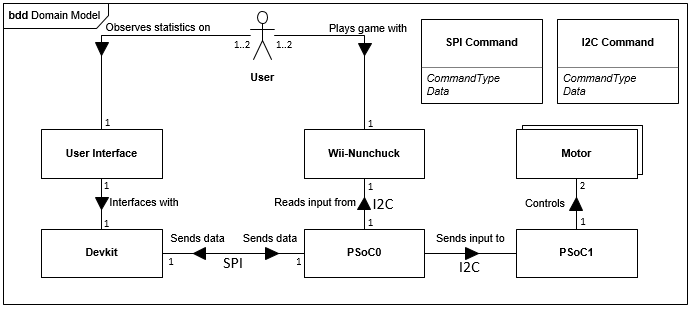
\includegraphics[width=\textwidth]{Systemarkitektur/images/DomainModel}
	\caption{Domæne model for Candygun 3000}
	\label{fig:DomainModel}
\end{figure}

I domæne modellen ses, at brugeren interagerer med både Wii-nunchucken og med brugergrænsefladen. Brugergrænsefladen er en grænseflade til softwaren devkittet. Devkittet kommunikerer med PSoC0, som læser den analoge data der kommer fra Wii-nunchucken. Denne data bliver derefter afkodet og videresendt til PSoC1, som styrer motorene ud fra dataene. PSoC1 sender også et interrupt til PSoC2, når 'Z' knappen på nunchucken bliver trykket. Når PSoC2 modtager interruptet, starter motoren for affyringsmekanismen i projectile launcher.


I "I2C Command" ses en grov estimering af interfacet mellem de forskellige I2C enheder i systemet. Commandtype bruges til at identificere hvilken data der bliver sendt. Data er en mængde tal-værdier der bliver tolket ud fra hvilken commandtype der er blevet sendt.

I "SPI Command" ses en estimering af interfacet mellem SPI enhederne i systemet. "Commandtype" bruges til at identificere hvilken opgave systemet skal udføre (f.eks. 'I2C-test'). Data kan indeholde tal-værdier, som repræsenterer nunchuck værdier (buttonpress osv.). 
En mere detaljeret gennemgang af disse kommunikations protokoller kan findes i afsnit \ref{afsnit:kommunikationsprotokoller} - Kommunikationsprotokoller.

% ---------------BDD--------------------------------------------------
\section{BDD for Candygun 3000}
På figur \ref{fig:BDD} ses et \textit{Block Definition Diagram (BDD)} 
Figur \ref{fig:BDD} skal give et overblik over hvordan  relationerne mellem de forskellige hardwareblokke er. Så man får et overordnet billede af hvordan strukturen er for ” Candygun 3000”. For at læse hvad hver blok skal bruges til, henvises der til tabel \ref{blokbeskrivelse} (blokbeskrivelse). Der på BDD'et figur \ref{fig:BDD} med nødvændige indgange og udgange for de fysiske signaler. Yderligere ses det at flow specifikationer er defineret for de ikke-atomare forbindelser \textit{I2C} samt \textit{SPI}, da disse er busser bestående af flere forbindelser. Der henvises til \textbf{IBD AFSNIT} for en detaljeret model af de fysiske forbindelser mellem hardwareblokkende.



\begin{figure}[H]
	\centering
	%trim = {1.8cm 14.6cm 1.8cm 1cm}, clip = true, %
	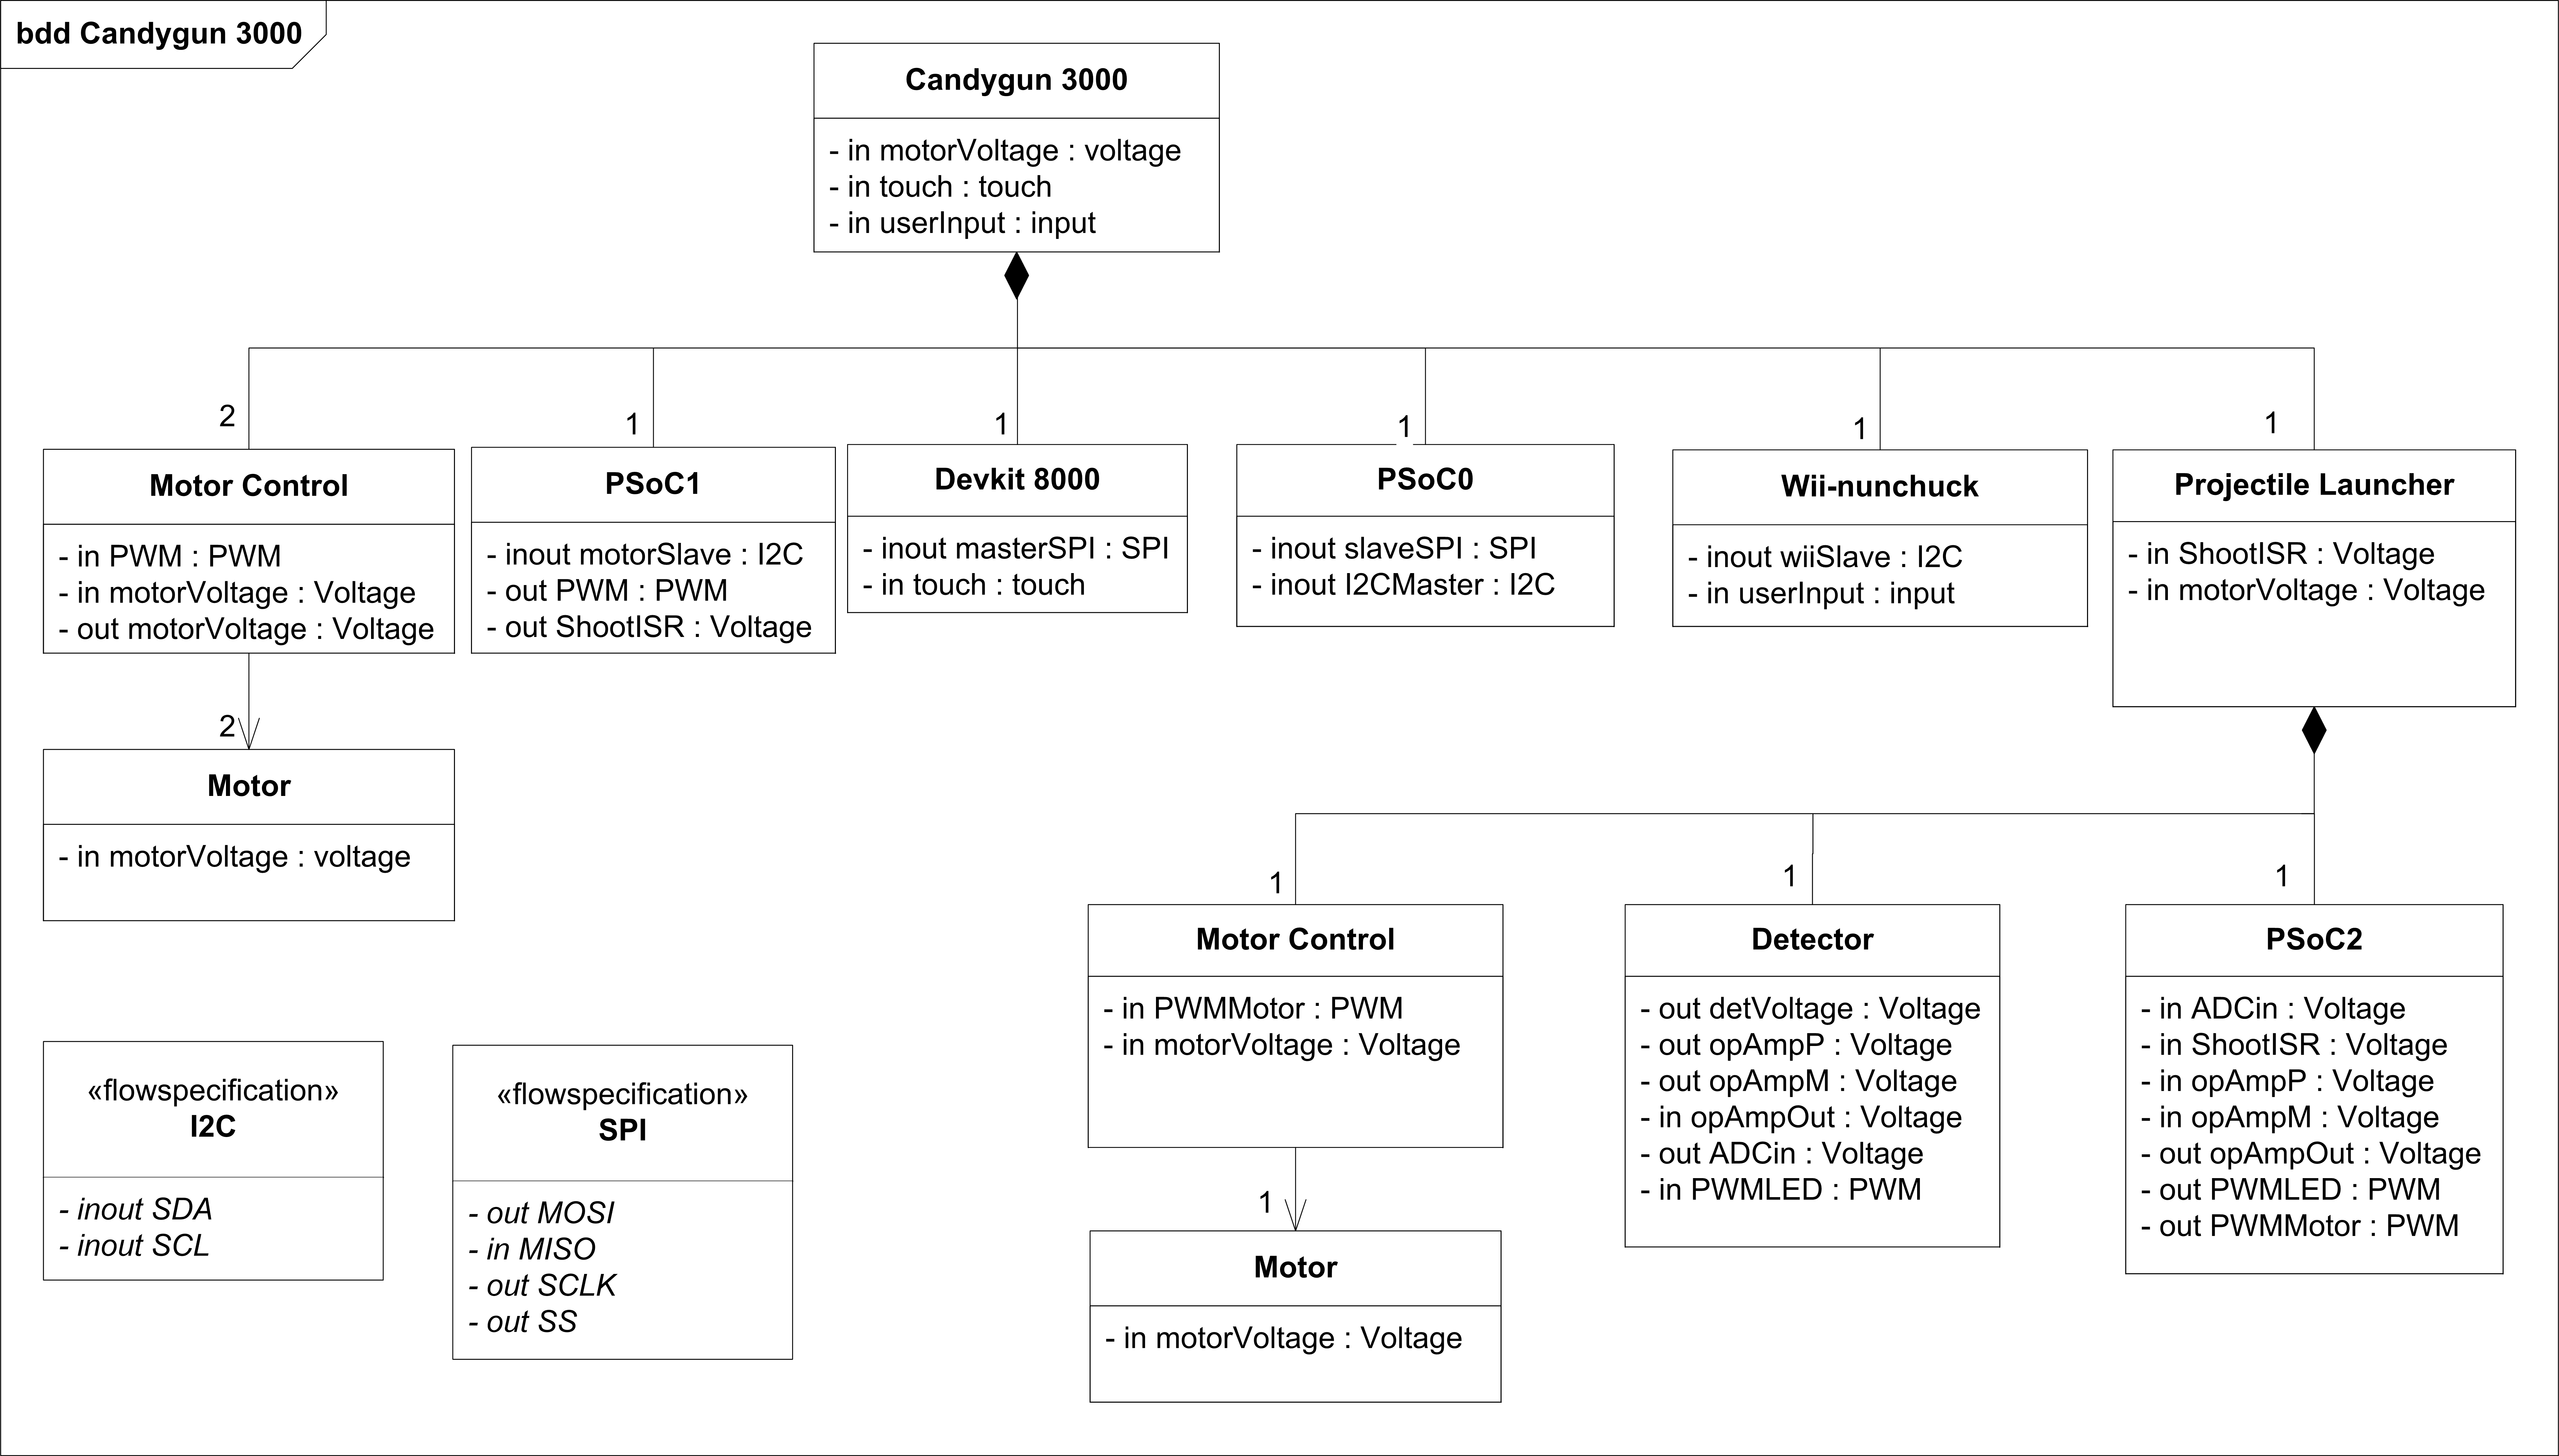
\includegraphics[width= \textwidth]{Systemarkitektur/images/BDD_overordnet1.png}
	\caption{BDD for Candygun 3000}
	\label{fig:BDD}
\end{figure}


\subsection{Blokbeskrivelse}
\begin{table}[H]
	\centering
	\begin{tabular}{|l|l|}
		\hline
		\textbf{Bloknavn}       & \textbf{Beskrivelse}                                                                                                                                                                                                                           \\ \hline
		Devkit 8000             & \begin{tabular}[c]{@{}l@{}}
			DevKit 8000 er en embedded Linux platform med touch-skærm, \\ der bruges tilbrugergrænsefladen for produktet. Brugeren inter- \\ agerer med systemet og ser status for spillet via Devkit 8000.                                                      \end{tabular} \\ \hline
		Wii-Nunchuck            & \begin{tabular}[c]{@{}l@{}}Wii-Nunchuck er controlleren som brugeren styrer kanonens \\ retning med. \end{tabular} \\ \hline
		PSoC0                   & \begin{tabular}[c]{@{}l@{}}PSoC0 er PSoC hardware der indeholder software til I2C og \\ SPI kommunikationen og afkodning af Wii-Nunchuck data. \\ PSoC0 fungerer som I2C masterog SPI slave. Denne PSoC er \\ bindeleddet mellem brugergrænsefladen og restenaf systemets \\ hardware. \end{tabular} \\ \hline
		MotorControl                   & \begin{tabular}[c]{@{}l@{}}MotorControl blokken er Candy Gun 3000’s motorerer, der anvendes \\ til at bevæge kanonen. Denne blok består af H-bro blokken og \\ rotationsbegrænsnings blokken. \end{tabular} \\ \hline
		Motor &
		\begin{tabular}[c]{@{}l@{}}Motor er motorene der bruge til at bevæge platform og kanon. \end{tabular} \\ \hline
		H-bro &
		\begin{tabular}[c]{@{}l@{}}H-bro bruges til at styre mototrens rotationsretning \end{tabular} \\ \hline
		Rotationsbegrænsning &
		\begin{tabular}[c]{@{}l@{}}Rotationsbegrænsning er til at begrænse platformens rotation så \\ denne ikke kan dreje 360 grader. Den blok består af et potentiometer \\ og en ADC'en, som sidder internt på PSoC0  \end{tabular} \\ \hline
		PSoC1                   & \begin{tabular}[c]{@{}l@{}}PSoC1 er PSoC hardware der indeholder software til I2C \\ kommunikation og styring af Candy Gun 3000’s motorer. \\ PSoC1 fungerer som I2C slave. \end{tabular} \\ \hline
		SPI (FlowSpecification) &  \begin{tabular}[c]{@{}l@{}}SPI (FlowSpecification) beskriver signalerne der indgår i SPI \\ kommunikation. \end{tabular} \\ \hline
		I2C (FlowSpecification) &  \begin{tabular}[c]{@{}l@{}}I2C (FlowSpecification) beskriver signalerne der indgår i I2C \\ kommunikation. \end{tabular} \\ \hline	
		Projectile Launcher  &  \begin{tabular}[c]{@{}l@{}} Affyringsmekanismen indeholder PSoC2, Motor Control Shoot, \\ Motor Shoot og Rotation Detector og sørger dermed for \\ affyring af kanonen.  \end{tabular} \\ \hline
		PSoC2  & \begin{tabular}[c]{@{}l@{}} PSoC2 indeholder en operationsforstærker til rotations-\\detektorkredsløbet, en ADC som aflæser rotationsdetektoren. \\ Derudover står den for at sende PWM-signaler til LED'en \\ i rotationsdetektoren og til motorstyringsblokken.   \end{tabular} \\ \hline
		Motor Control Shoot  &  \begin{tabular}[c]{@{}l@{}} Denne blok står for at styre affyringsmekanismens motor.  \end{tabular} \\ \hline
		Motor Shoot  &  \begin{tabular}[c]{@{}l@{}} Motor Shoot er motoren, der sidder i affyringsmekanismen.  \end{tabular} \\ \hline
		Rotation Detector  &  \begin{tabular}[c]{@{}l@{}} Rotationsdetekoren detekterer, at der er blevet affyret et stykke \\ slik og sender et signal til PSoC2 om dette. \end{tabular} \\ \hline
	\end{tabular}
	\label{blokbeskrivelse}
	\caption{Blokbeskrivelse}
\end{table} 

%---------------IBD--------------------------------------------------
\section{IBD for Candygun 3000}
På baggrund af BDD'et er der lavet et \textit{Internal Block Diagram (IBD)}. I IBD'et på figur \ref{fig:IBD} ses forbindelserne og portene mellem systemets blokke. Diagrammet viser grænsefladerne mellem blokkene og flowet i mellem disse. 

\begin{figure}[H] 
	\begin{adjustwidth}{-3cm}{-\rightmargin}
		\centering
		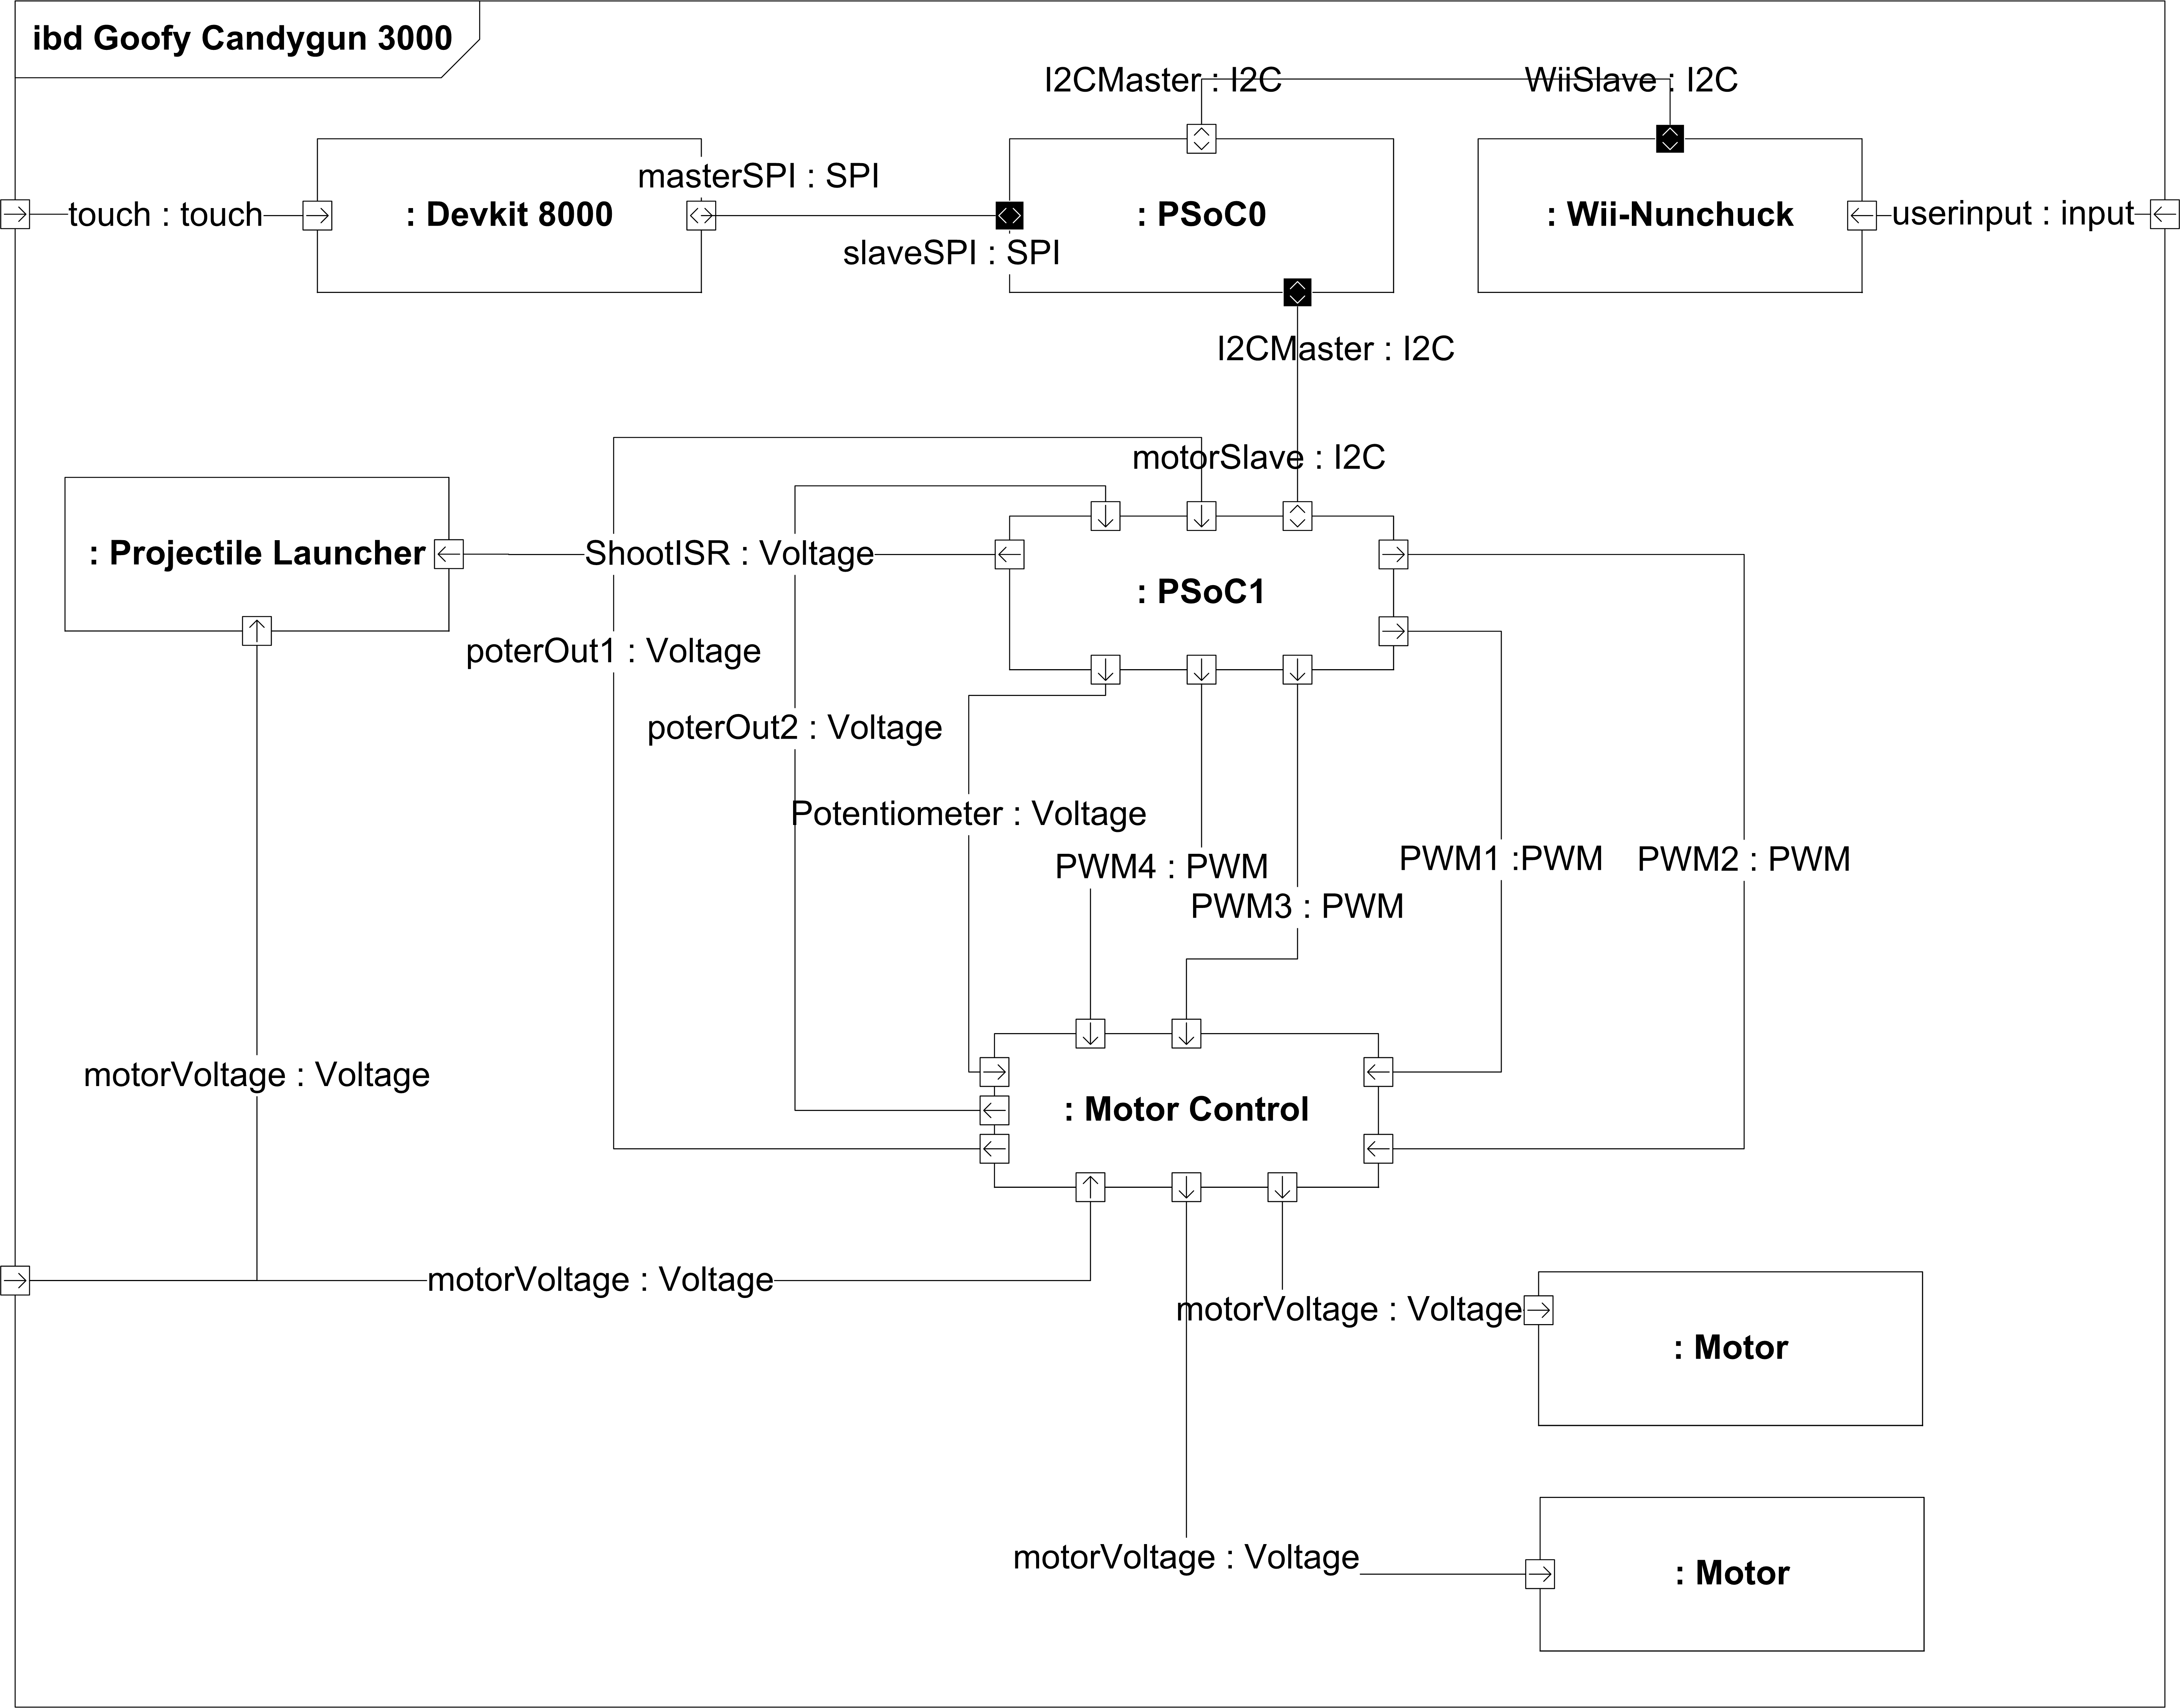
\includegraphics[width=0.85\paperwidth]{Systemarkitektur/images/IBD_V4}		
	\end{adjustwidth}
	\caption{IBD for Candygun 3000}
	\label{fig:IBD}
\end{figure}

I IBD'et på figur \ref{fig:IBDm} ses forbindelserne og portene mellem blokkene i motorControl blokken. Diagrammet viser grænsefladerne mellem disse blokke og flowet i mellem disse.

\begin{figure}[H]
	\centering
	%trim = {1.8cm 14.6cm 1.8cm 1cm}, clip = true, %
	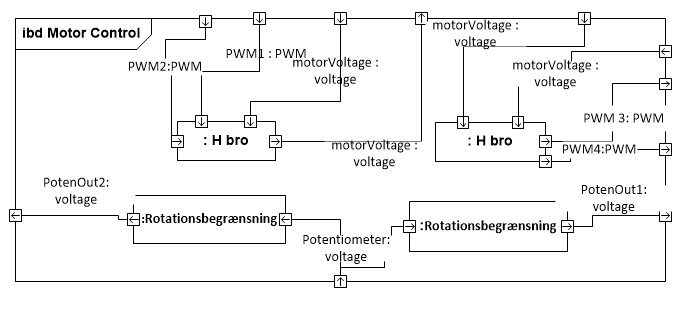
\includegraphics[width= \textwidth]{Systemarkitektur/images/IBDmotorcontrol2}
	\caption{IBD for motor control}
	\label{fig:IBDm}
\end{figure}

På figur \ref{fig:IBDaffyring} ses et IBD, der giver et overblik over affyringsmekanismens ind- og udgående signaler og forbindelserne mellem de interne blokke, som udgør affyringsmekanismen. 

\begin{figure}[H]
	\centering
	%trim = {1.8cm 14.6cm 1.8cm 1cm}, clip = true, %
	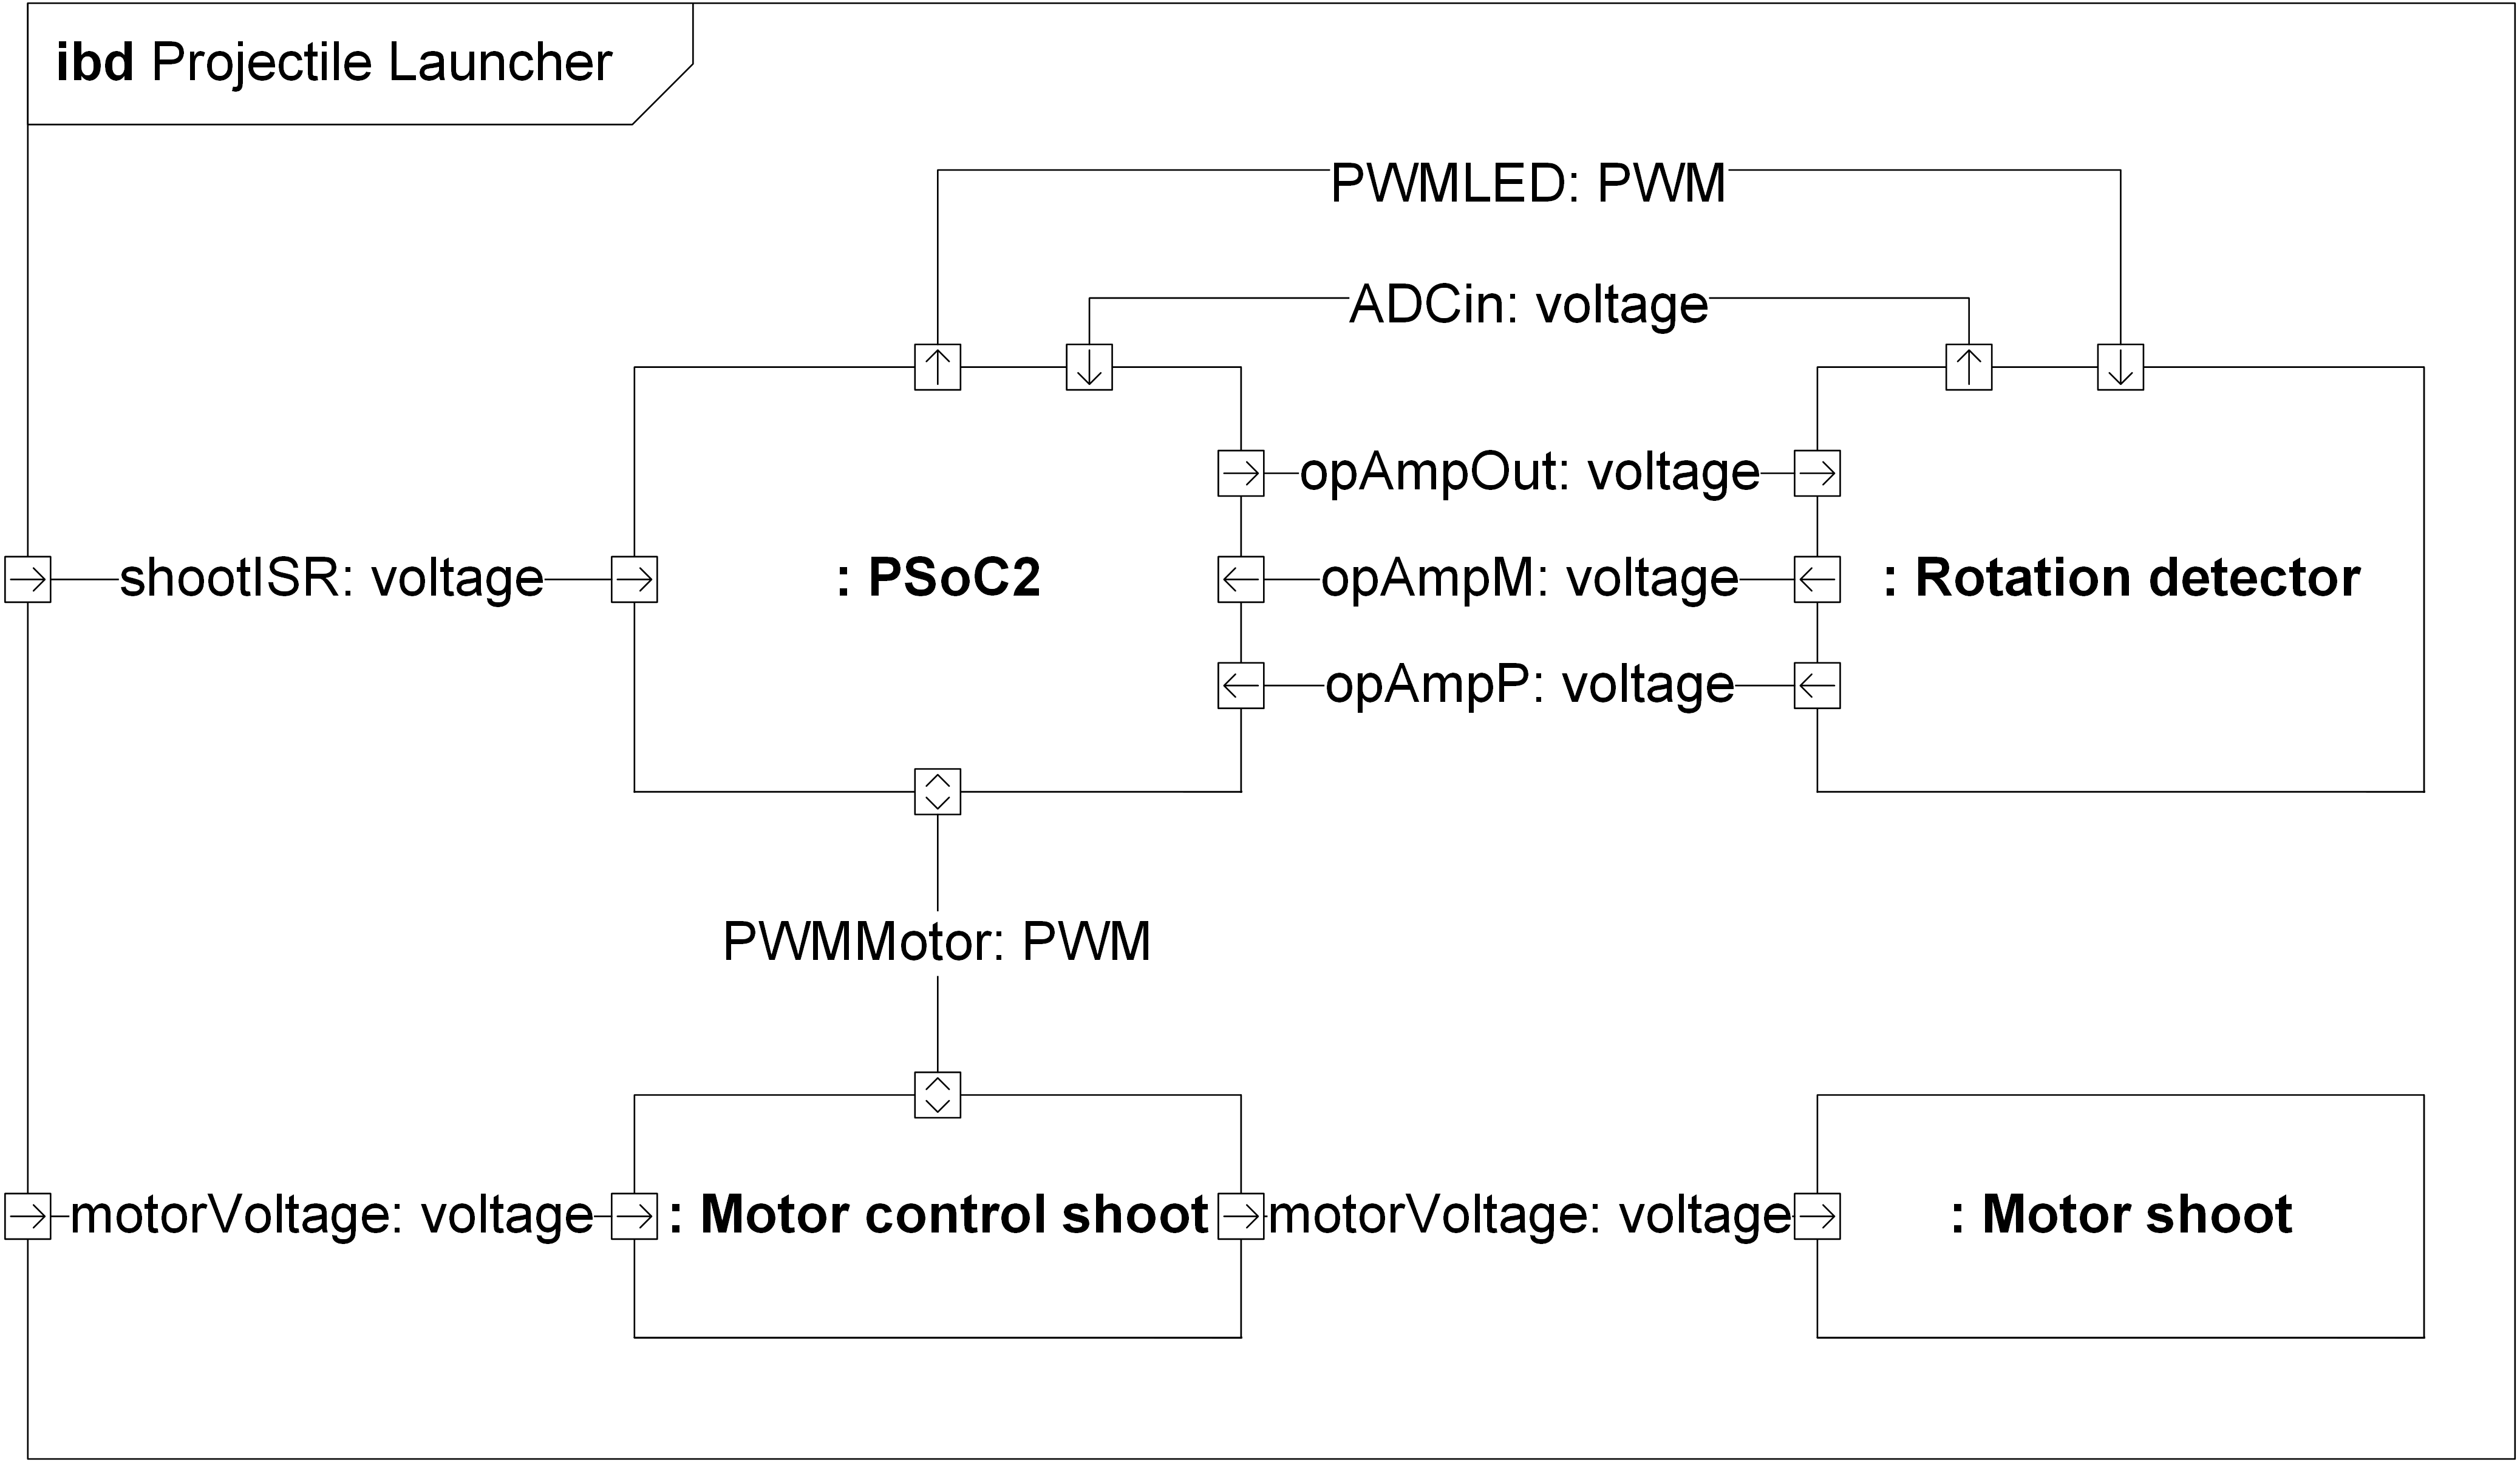
\includegraphics[width= \textwidth]{Systemarkitektur/images/IBDaffyring}
	\caption{IBD over affyringsmekanismen}
	\label{fig:IBDaffyring}
\end{figure}

I tabel \ref{signalbeskrivelse} ses en beskrivelse af alle signaler, der indgår i de tre IBD'er, som ses på figurerne \ref{IBD}, \ref{IBDm} og \ref{IBDaffyring}. 

\subsection{Signalbeskrivelse}

I signalbeskrivelsen gælder det, at når et signal beskrives som 'højt' opereres der i et spændingsområde på 3.5V til 5V. På samme måde er signaler beskrevet som 'lav' defineret som spændinger indenfor et område fra 0V til 1,5V. Disse spændingsniveauer er defineret  ud fra standarden for CMOS kredse \cite{cmosStandard}.
\begin{longtable}{|>{\hspace{0pt}}p{3cm} | >{\hspace{0pt}}p{3cm} | p{2cm} | p{3cm} |}
	\hline                                                                                                                                                         
	\textbf{Blok-navn} & \textbf{Funktionsbeskrivelse} & \textbf{Signaler} & \textbf{Signalbeskrivelse} \\ \hline
	Devkit 8000 & Fungerer som grænseflade mellem bruger og systemet samt SPI master. & masterSPI & Type: SPI \newline Spændingsniveau: 0-5V \newline Hastighed: 1Mbps \newline Beskrivelse: SPI bussen hvori der sendes og modtages data.\\ \cline{3-4}
	& & touch & Type: touch \newline Beskrivelse: Brugertryk på Devkit 8000 touchdisplay. \\ \hline
	PSoC0 & Fungerer som I2C master for PSoC1 og Wii-Nunchuck samt SPI slave til Devkit 8000. & slaveSPI & Type: SPI \newline Spændingsniveau: 0-5V \newline Hastighed: 1Mbps \newline Beskrivelse: SPI bussen hvori der sendes og modtages data.\\ \cline{3-4}
	& & wiiMaster & Type: I2C \newline Spændingsniveau: 0-5V\newline Hastighed: 100Kpbs \newline Beskrivelse: I2C bussen hvor der modtages data fra Nunchuck.\\ \cline{3-4}
	& & motorMaster & Type: I2C \newline Spændingsniveau: 0-5V \newline Hastighed: 100kbit/sekund \newline Beskrivelse: I2C bussen hvor der sendes afkodet Nunchuck data til PSoC1.\\ \hline
	PSoC1 & Modtager nunchuckinput fra PSoC0 og omsætter dataene til PWM signaler. & motorSlave & Type: I2C \newline Spændingsniveau: 0-5V \newline Hastighed: 100kbit/sekund \newline Beskrivelse: Indeholder formatteret Wii-Nunchuck data som omsættes til PWM-signal. \\ \cline{3-4} 
	&& ShootISR & Type: voltage \newline Spændingsniveau: 0-5V \newline Beskrivelse:  giv et højt signal når den skal skyde.\\ \cline{3-4}   
	& & PWM & Type: PWM \newline Frekvens: 22kHz \newline PWM \%: 0-100\% \newline Spændingsniveau: 0-5V \newline Beskrivelse: PWM signal til styring af motorens hastighed. \\ \cline{3-4}
	& & PotenOut1 & Type: voltage \newline Spændingsniveau: en spænding 0V-5V alt efter hvad potentiometer står på \newline Beskrivelse: den spænding viser hvor motoren står henne\\ \cline{3-4}
	& & PotenOut2 & Type: voltage \newline Spændingsniveau: en spænding 0V-5V alt efter hvad potentiometer står på \newline Beskrivelse: den spænding viser hvor motoren står henne\\ \cline{3-4}
	& & PWM1 & Type: PWM \newline Frekvens: 3MHz \newline PWM\%: 0-100\% \newline Spædingsniveau: 0-5V \newline Beskrivelse: PWM signal til styring af motorens hastighed. \\ \cline{3-4}
	&& PWM2 & Type: PWM \newline Frekvens: 3MHz \newline PWM\%: 0-100\% \newline Spædingsniveau: 0-5V \newline Beskrivelse: PWM signal til styring af motorens hastighed. \\ \cline{3-4}
	
	
	&& PWM3 & Type: PWM \newline Frekvens: 3MHz \newline PWM\%: 0-100\% \newline Spædingsniveau: 0-5V \newline Beskrivelse: PWM signal til styring af motorens hastighed. \\ \cline{3-4}
	&& PWM4 & Type: PWM \newline Frekvens: 3MHz \newline PWM\%: 0-100\% \newline Spædingsniveau: 0-5V \newline Beskrivelse: PWM signal til styring af motorens hastighed. \\ \cline{3-4}
	& & motorVoltage & Type: voltage \newline Spændingsniveau: 9V \newline Beskrivelse: Strømforsyning til motoren\\ \cline{3-4}
	& & potentiometer & Type: voltage \newline Spændingsniveau: 5V \newline Beskrivelse: giver Rotationsbegrænsing 5V \\ \hline
	MotorControl & Den enhed der skal bevæge kanonen & PWM1 & Type: PWM \newline Frekvens: 3MHz \newline PWM\%: 0-100\% \newline Spædingsniveau: 0-5V \newline Beskrivelse: PWM signal til styring af motorens hastighed. \\ \cline{3-4}
	&& PWM2 & Type: PWM \newline Frekvens: 3MHz \newline PWM\%: 0-100\% \newline Spædingsniveau: 0-5V \newline Beskrivelse: PWM signal til styring af motorens hastighed. \\ \cline{3-4}
	
	
	&& PWM3 & Type: PWM \newline Frekvens: 3MHz \newline PWM\%: 0-100\% \newline Spædingsniveau: 0-5V \newline Beskrivelse: PWM signal til styring af motorens hastighed. \\ \cline{3-4}
	&& PWM4 & Type: PWM \newline Frekvens: 3MHz \newline PWM\%: 0-100\% \newline Spædingsniveau: 0-5V \newline Beskrivelse: PWM signal til styring af motorens hastighed. \\ \cline{3-4}
	& & motorVoltage & Type: voltage \newline Spændingsniveau: 9V \newline Beskrivelse: Strømforsyning til motoren\\ \cline{3-4}
	& & potentiometer & Type: voltage \newline Spændingsniveau: 5V \newline Beskrivelse: giver Rotationsbegrænsing 5V 
	\\ \cline{3-4}
	& & PotenOut1 & Type: voltage \newline Spændingsniveau: en spænding 0V-5V alt efter hvad potentiometer står på \newline Beskrivelse: den spænding viser hvor motoren står henne\\ \cline{3-4}
	& & PotenOut2 & Type: voltage \newline Spændingsniveau: en spænding 0V-5V alt efter hvad potentiometer står på \newline Beskrivelse: den spænding viser hvor motoren står henne
	\\ \hline
	Motor & Denne blok beskriver, hvad motoren får. & Motorvoltage & Type: voltage \newline Spændingsniveau: 0-5V  \newline Beskrivelse: giver spændning til motoren.(denne beskevelse glæder også for den anden motor) \\ \hline
	Wii-nunchuck & Den fysiske controller som brugeren styrer kanonen med. & wiiSlave & Type: I2C \newline Spændingsniveau: 0-5V \newline Hastighed: 100kbit/sekund \newline Beskrivelse: Kommunikationslinje mellem PSoC1 og Wii-Nunchuck. \\ \cline{3-4}
	& & userInput & Type: input \newline Beskrivelse: Brugerinput fra Wii-Nunchuck. \\ \hline
	SPI & Denne blok beskriver den ikke-atomiske SPI forbindelse. & MOSI & Type: CMOS \newline Spændingsniveau: 0-5V \newline Beskrivelse: Binært data der sendes fra master til slave. \\ \cline{3-4}
	& & MISO & Type: CMOS \newline Spændingsniveau: 0-5V \newline Beskrivelse: Binært data der sendes fra slave til master. \\ \cline{3-4}
	& & SCLK & Type: CMOS \newline Spændingsniveau: 0-5V \newline Hastighed: 1Mbps\newline Beskrivelse: Clock signalet fra master til slave, som bruges til at synkronisere den serielle kommunikation. \\ \cline{3-4}
	& & SS & Type: CMOS \newline Spændingsniveau: 0-5V \newline  Beskrivelse: Slave-Select, som bruges til at bestemme hvilken slave der skal kommunikeres med. \\ \hline
	I2C & Denne blok beskriver den ikke-atomiske I2C forbindelse. & SDA & Type: CMOS \newline Spændingsniveau: 0-5V \newline \newline Beskrivelse: Databussen mellem I2C masteren og I2C slaver. \\ \cline{3-4}
	& & SCL & Type: CMOS \newline Spændingsniveau: 0-5V \newline Hastighed: 100kbps \newline Beskrivelse: Clock signalet fra master til lyttende I2C slaver, som bruges til at synkronisere den serielle kommunikation. \\ \hline
	
	Projectile Launcher & Denne blok består blokkene PSoC2, Detector og Motor Control Shoot & shootISR & Type: Voltage \newline Spændingsniveau: 0-5V \newline \newline Beskrivelse: Giv et højt signal, når kanonen skal skyde. \\ \cline{3-4}
	& & motorVoltage & Type: Voltage \newline Spændingsniveau: 9V \newline Beskrivelse: Strømforsyning til motor.  \\ \hline
	
	PSoC2 & Aflæser signaler fra rotationsdetektor og udsender PWM-signal til LED og Motor Shoot. & ADCin & Type: Voltage \newline Spændingsniveau: 0,5-5V \newline  \newline Beskrivelse: Rotationsdektors output som aflæses af ADC på PSoC2.  \\ \cline{3-4}
	& & shootISR & Type: Voltage \newline Spændingsniveau: 0-5V \newline Beskrivelse: Giver et højt signal, når motoren skal skyde. \\ \cline{3-4}
	& & opAmpP & Type: Voltage \newline Spændingsniveau: 0,5V \newline Beskrivelse: Referencespænding til operationsforstærkerens positive indgang. \\ \cline{3-4}
	& & opAmpM & Type: Voltage \newline Spændingsniveau: 0,5V \newline Beskrivelse: Virtuelt nul. Den ligger altid på 0,5V pga. negativ feedback på operationsforstærkeren. \\ \cline{3-4}
	& & opAmpOut & Type: Voltage \newline Spændingsniveau: 0,5-5V \newline Beskrivelse: Udgang på operationsforstærker i rotationsdetektorkredsløbet. \\ \cline{3-4}
	& & PWMLED & Type: PWM \newline Spændingsniveau: 0-5V \newline Frekvens: 10kHz \newline PWM\%: 0-100\% \newline Beskrivelse: Udsender PWM-signal til LED'en i rotationsdetektorkredsløbet. \\ \cline{3-4}
	& & PWMMotor & Type: PWM \newline Spændingsniveau: 0-5V \newline Frekvens: 33,33kHz \newline PWM\%: 0-100\% \newline Beskrivelse: Udsender PWM-signal til LED'en i rotationsdetektorkredsløbet. \\ \hline
	
	Detector & Rotationsdetektoren detekterer om der er skudt. & opAmpP & Type: Voltage \newline Spændingsniveau: 0,5V \newline Beskrivelse: Referencespænding til operationsforstærkerens positive indgang. \\ \cline{3-4}
	& & opAmpM & Type: Voltage \newline Spændingsniveau: 0,5V \newline Beskrivelse: Virtuelt nul. Den ligger altid på 0,5V pga. negativ feedback på operationsforstærkeren. \\ \cline{3-4}
	& & opAmpOut & Type: Voltage \newline Spændingsniveau: 0,5-5V \newline Beskrivelse: Udgang på operationsforstærker i rotationsdetektorkredsløbet. \\ \cline{3-4}
	& & ADCin & Type: Voltage \newline Spændingsniveau: 0,5-5V \newline  \newline Beskrivelse: Rotationsdektors output som aflæses af ADC på PSoC2.  \\ \cline{3-4}
	& & PWMLED & Type: PWM \newline Spændingsniveau: 0-5V \newline Frekvens: 10kHz \newline PWM\%: 0-100\% \newline Beskrivelse: Udsender PWM-signal til LED'en i rotationsdetektorkredsløbet. \\ \hline
	
	Motor Control Shoot & Denne blok styrer Motor Shoot til affyringsmekanismen. & PWMMotor & Type: PWM \newline Spændingsniveau: 0-5V \newline Frekvens: 33,33kHz \newline PWM\%: 0-100\% \newline Beskrivelse: Udsender PWM-signal til LED'en i rotationsdetektorkredsløbet. \\ \cline{3-4}
	& & motorVoltage & Type: Voltage \newline Spændingsniveau: 9V \newline Beskrivelse: Strømforsyning til motor. \\ \hline 
	
	Motor Shoot & Denne blok er affyringsmekanismens motor. & motorVoltage & Type: Voltage \newline Spændingsniveau: 9V \newline Beskrivelse: Strømforsyning til motor. \\ \hline 	
	\caption{Signalbeskrivelse}
	\label{signalbeskrivelse} 
\end{longtable}


\section{Software Allokeringsdiagram}
På figur \ref{fig:softwareAllocation} ses et software allokations diagram. Dette diagram danner et overblik over hvilke CPU'er der findes i systemet, og hvilken software der skal allokeres på disse. Følgende applikationsmodeller tager udgangspunkt i softwaren der allokeres i figuren.

\begin{figure}[H]
	\centering
	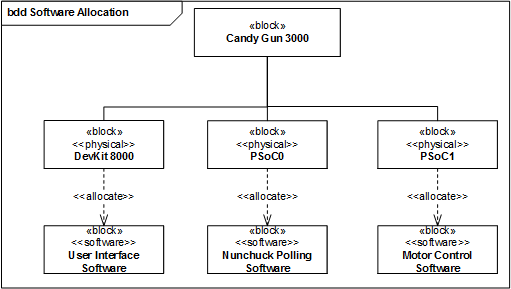
\includegraphics[width=\textwidth]{Systemarkitektur/images/SoftwareAllocation.png}
	\caption{Software allokations diagram}
	\label{fig:softwareAllocation}
\end{figure}

På tabel \ref{tabel:softwareAllocationDescription} er hvert allokeret software komponent beskrevet.

\begin{table}[H]
	\centering
	\begin{tabular}{|ll|}
		\hline
		User Interface Software   & \begin{tabular}[c]{@{}l@{}}Dette allokerede software er brugergrænsefladen\\ som brugeren interagerer med på DevKit8000 touch-skærmen.\end{tabular}                                                  \\
		\rowcolor[HTML]{CBCEFB} 
		Nunchuck Polling Software & \begin{tabular}[c]{@{}l@{}}Dette allokerede software har til ansvar at polle\\ Nunchuck tilstanden og videresende det til\\ PSoC1.\end{tabular}                                                      \\
		Motor Control Software    & \cellcolor[HTML]{FFFFFF}\begin{tabular}[c]{@{}l@{}}Dette allokerede software har til ansvar at\\ bruge den pollede Nunchuck data fra PSoC0\\ til motorstyring samt affyringsmekanismen.\end{tabular} 
		\\ 
		\rowcolor[HTML]{CBCEFB} 
		Projectile Launcher Software & \begin{tabular}[c]{@{}l@{}}Dette allokerede software har til ansvar at aktivere\\ affyringsmekanismen når et \\ knaptryk detekteres på Nunchuck.\end{tabular} \\
		\hline
	\end{tabular}
	\caption{Beskrivelse af den allokerede software}
	\label{tabel:softwareAllocationDescription}
\end{table}

\section{Applikationsmodeller}
Til arkitekturfasen er der gjort brug af applikationsmodeller som et analyseværktøj. Der er lavet en applikationsmodel for hver use case, for hvert software komponent identificeret i Software Allokeringsdiagrammet, tabel \ref{tabel:softwareAllocationDescription}. Hver applikationsmodel består af et \textit{Klasse Identifikations Diagram}, \textit{Sekvensdiagram} og \textit{Klassediagram}. Resultatet af hver applikationsmodel er et klassediagram der indeholder konceptuelle klasser med metoder relevant for den pågældende use case. \newline

\noindent Med konceptuelle klasser menes der at de ikke nødvændigvis behøver at have et 1:1 forhold med de implementerede klasser. De konceptuelle klasser bruges som inspiration til de klasser og funktioner der muligvis skal modelleres i projektets problemdomæne. 

\subsection{Use Case 1 - Spil Goofy Candy Gun 3000}

Følgende afsnit præsenterer applikationsmodeller relevante til Use Case 1 - Spil Goofy Candy Gun 3000, fordelt over systemets CPU'er.

På figur \ref{fig:WiiNunchuckSequenceDiagram} ses et overordnet sekvensdiagram for hvordan Nunchuck data bliver overført igennem systemet og påvirker motorer samt affyringsmekanismen.

\begin{figure}[H]
	\centering
	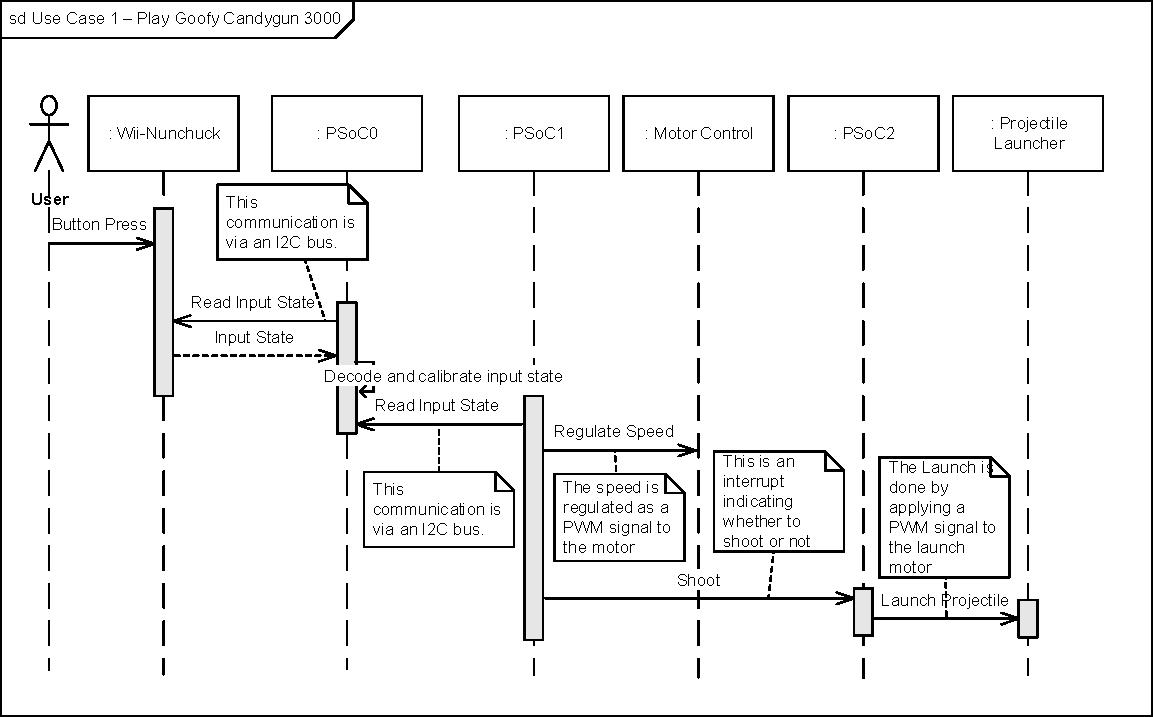
\includegraphics[width=\textwidth]{Systemarkitektur/images/SequenceDiagramUC1}
	\caption{Overordnet sekvensdiagram for Wii-Nunchuck informations flow}
	\label{fig:WiiNunchuckSequenceDiagram}
\end{figure}

\subsubsection{Applikationsmodel for Nunchuck Polling Software}

\begin{figure}[H]
	\centering
	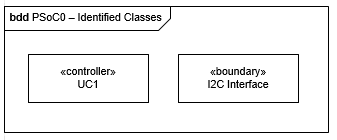
\includegraphics[scale=0.8]{Systemarkitektur/images/klasseIdentificationUC1PSoC0}
	\caption{Klasseidentifikation for PSoC0}
	\label{fig:klasseidentifikationUC1PSoC0}
\end{figure}

På figur \ref{fig:klasseidentifikationUC1PSoC0} ses klasse identifikation for Nunchuck Polling Software. Der er til Nunchuck Polling Software for Use Case 1 identificeret to klasser: \textit{UC1} samt \textit{I2C Interface}. \newline

\noindent Klassen \textit{UC1} er en controller. Dette er klassen der har til ansvar at eksekvere funktionalitet relevant til use case 1. \textit{I2C Interface} er en boundary klasse der repræsenterer grænseflade til I2C bussen.

Det kan på sekvensdiagrammet, figur \ref{fig:sekvensUC1PSoC0}, ses hvordan klasserne interagerer med hinanden. Her kan det ses at klassen \textit{UC1} aflæser Nunchuck input og herefter dekoder det, kalibrerer det, og sender det videre ud på I2C bussen hvor andre slaver kan gøre brug af dataen.

\begin{figure}[H]
	\centering
	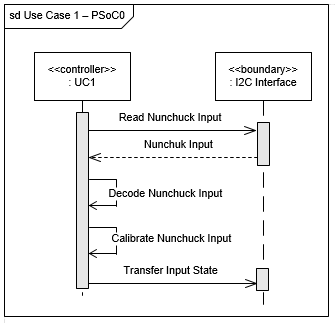
\includegraphics[scale=0.8]{Systemarkitektur/images/UC1PSoC0SequenceDiagram}
	\caption{Sekvensdiagram for PSoC0}
	\label{fig:sekvensUC1PSoC0}
\end{figure}

Figur \ref{fig:klasseUC1PSoC0} viser et endeligt klassediagram, hvor metoderne er udledt fra sekvensdiagrammet, figur \ref{fig:sekvensUC1PSoC0}. Her er det identificeret at controller klassen \textit{UC1} har to metoder til at kunne dekode og kalibrere Nunchuck data. \textit{UC1} gør brug af \textit{I2C Interface} som grænseflade til at sende dataen ud på I2C bussen.

\begin{figure}[H]
	\centering
	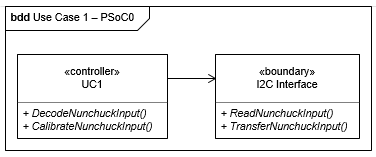
\includegraphics[scale=0.8]{Systemarkitektur/images/klasseUC1PSoC0}
	\caption{Klassediagram for PSoC0}
	\label{fig:klasseUC1PSoC0}
\end{figure}

\subsubsection{Applikationsmodel for Motor Control Software}

\begin{figure}[H]
	\centering
	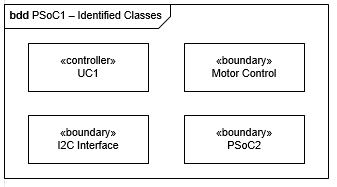
\includegraphics[scale=0.8]{Systemarkitektur/images/klasseIdentificationUC1PSoC1}
	\caption{Klasseidentifikation for PSoC1}
	\label{fig:klasseidentifikationUC1PSoC1}
\end{figure}

På figur \ref{fig:klasseidentifikationUC1PSoC1} ses klasse identifikation for Motor Control Software. Der er til Motor Control Software for Use Case 1 identificeret fire klasser: \textit{UC1}, \textit{Motor Control}, \textit{I2C Interface} og \textit{PSoC2}. \newline

\noindent \textit{UC1} er en controller. Denne klasse har til ansvar at eksekvere funktionalitet relevant til use case 1. \textit{Motor Control} repræsenterer grænsefladen til motorstyringen. \textit{I2C Interface} repræsenterer grænsefladen til I2C bussen. \textit{PSoC2} repræsenterer en grænseflade til PSoC2.

På figur \ref{fig:sekvensUC1PSoC1} ses et sekvensdiagram af interaktionen mellem disse klasser. Her kan det ses at \textit{UC1} klassen læser input data fra Nunchuck og videresender det til motor styringen samt PSoC2, så farten af motoren kan regulares og affyringsmekanismen kan aktiveres.

\begin{figure}[H]
	\centering
	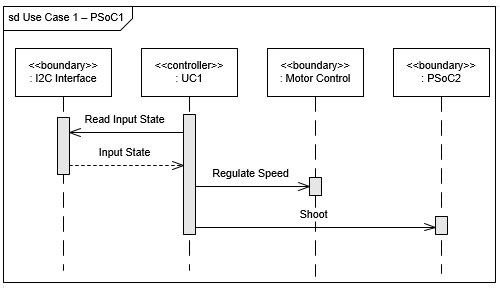
\includegraphics[scale=0.8]{Systemarkitektur/images/UC1PSoC1SequenceDiagram}
	\caption{Sekvensdiagram for PSoC1}
	\label{fig:sekvensUC1PSoC1}
\end{figure}

På figur \ref{fig:klasseUC1PSoC1} ses et endeligt klassediagram, hvor metoderne er udledt fra sekvensdiagrammet, figur \ref{fig:sekvensUC1PSoC1}. Her er det identificeret at controller klassen \textit{UC1} har primært kommunikerer med grænsefladerne \textit{I2C Interface}, \textit{PSoC2} og \textit{Motor Control}. Her skal \textit{UC1} kunne læse Nunchuck input fra \textit{I2C Interface}. Yderligere skal den kunne regulere farten på \textit{Motor Control} og affyre affyringsmekanismen.

\begin{figure}[H]
	\centering
	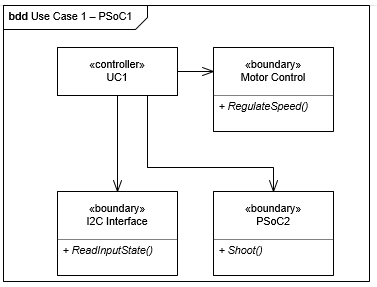
\includegraphics[scale=0.8]{Systemarkitektur/images/klasseUC1PSoC1}
	\caption{Klassediagram for PSoC1}
	\label{fig:klasseUC1PSoC1}
\end{figure}

\subsubsection{Applikationsmodel for Projectile Launcher Software}

\begin{figure}[H]
	\centering
	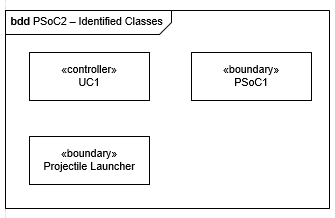
\includegraphics[scale=0.8]{Systemarkitektur/images/klasseIdentificationUC1PSoC2}
	\caption{Klasseidentifikation for PSoC2}
	\label{fig:klasseidentifikationUC1PSoC2}
\end{figure}

På figur \ref{fig:klasseidentifikationUC1PSoC2} ses klasse identifikation for Projectile Launcher Software. Der er til Projectile Launcher Software for use case 1 identificeret tre klasser: \textit{UC1}, \textit{PSoC1} og \textit{Projectile Launcher}.

\textit{UC1} er en controller. Denne klasse har til ansvar at eksekvere funktionaliteten relevant til use case 1. \textit{PSoC1} repræsenterer en grænseflade til PSoC1. \textit{Projectile Launcher} repræsenterer en grænseflade til affyringsmekanismen.

På figur \ref{fig:sekvensUC1PSoC2} ses et sekvensdiagram der viser klassernes interaktion. Her kan det ses at PSoC1 sender et signal til controlleren når der skal affyres et skud. Når dette signal er modtaget, bliver et aktiverings signal sendt ud til affyringsmekanismen.

\begin{figure}[H]
	\centering
	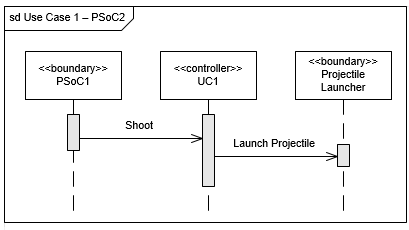
\includegraphics[scale=0.8]{Systemarkitektur/images/UC1PSoC2SequenceDiagram}
	\caption{Sekvensdiagram for PSoC2}
	\label{fig:sekvensUC1PSoC2}
\end{figure}

På figur \ref{fig:klasseUC1PSoC2} ses det endelige klassediagram, hvor metoderne er udledt fra sekvensdiagrammet, figur \ref{fig:sekvensUC1PSoC2}. Det kan her ses \textit{PSoC1} grænsefladen skal kunne sende en affyringsbesked til \textit{UC1}. \textit{UC1} skal derefter kunne aktivere affyringsmekanismen. 

\begin{figure}[H]
	\centering
	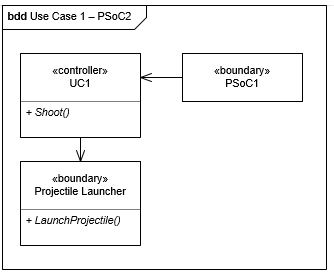
\includegraphics[scale=0.8]{Systemarkitektur/images/klasseUC1PSoC2}
	\caption{Klassediagram for PSoC2}
	\label{fig:klasseUC1PSoC2}
\end{figure}

\newpage
\subsection{Use Case 2 - Test Kommunikationsprotokoller}

Følgende afsnit præsenterer applikationsmodeller relevante til Use Case 2 - Test Kommunikationsprotokoller, fordelt over systemets CPU'er.

På figur \ref{fig:SystemTestOverviewSequenceDiagram} ses et overordnet sekvensdiagram for use casen. Her starter brugeren testen gennem brugergrænsefladen. Først bliver SPI bussen mellem DevKit8000 og PSoC0 testet. Herefter bliver I2C bussen testet ved at PSoC0 undersøger om de nødvændige I2C slaver (PSoC1 og Wii-Nunchuck) kan kommunikeres med. Til slut får brugeren en besked om at skulle trykke på en Wii-Nunchuck knap, hvorefter der bliver testet om knaptrykket skete eller ej.

\begin{figure}[H]
	\centering
	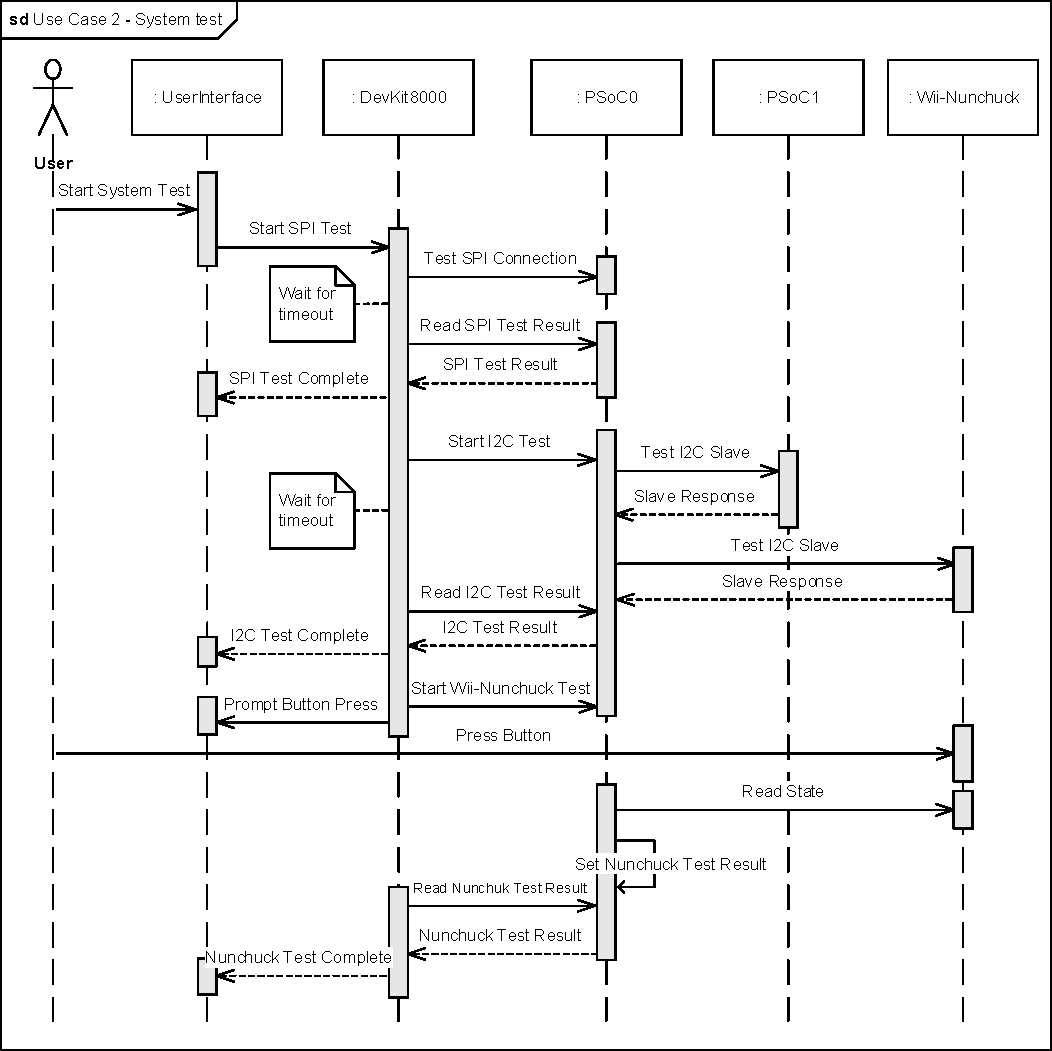
\includegraphics[width=\textwidth]{Systemarkitektur/images/SequenceDiagramUC2}
	\caption{Sekvensdiagram for Use Case 2 - Test Kommunikationsprotokoller}
	\label{fig:SystemTestOverviewSequenceDiagram}
\end{figure}

% ---------------Devkit Applikationsmodel-----------------------------
\subsubsection{Applikationsmodel for User Interface Software}

\begin{figure}[H]
	\centering
	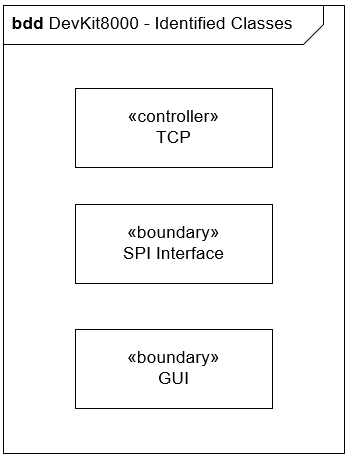
\includegraphics[scale=0.8]{Systemarkitektur/images/KlasseIdentifikationDevKit.png}
	\caption{Klasseidentifikation for Devkit 8000}
	\label{fig:klasseidentifikationDevKit}
\end{figure}

På figur \ref{fig:klasseidentifikationDevKit} ses klasse identifikation for User Interface Software. Der er til User Interface Software for use case 2 identificeret tre klasser: \textit{Test Communication Protocol (TCP)}, \textit{SPI Interface}, og \textit{GUI}.

\textit{TCP} er en controller. Denne klasse har til ansvar at eksekvere funktionalitet relevant til use case 2. \textit{SPI Interface} repræsenterer en grænseflade til systemets SPI bus. \textit{GUI} repræsenterer en grænseflade til systemets grænseflade.

På figur \ref{fig:sekvensDevkit} ses et sekvensdiagram der viser klassernes interaktion. Som det fremkommer af diagrammet er det \textit{TCP} klassen, der sørger for, at de forskellige tests bliver sat i gang ved at kommunikere med PSoC0 over SPI bussen via \textit{SPI Interface} klassen. Når en test er færdiggjort meldes resultatet ud til brugeren via GUI'en.

\begin{figure}[H]
	\centering
	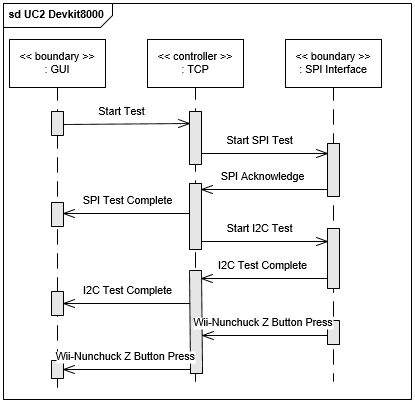
\includegraphics[]{Systemarkitektur/images/DevKit8000SequenceDiagram.png}
	\caption{Sekvensdiagram for Devkit 8000}
	\label{fig:sekvensDevkit}
\end{figure}

Ud fra sekvensdiagrammet, figur \ref{fig:sekvensDevkit}, er der udledt metoder til klasserne. De udledte metoder ses i klassediagrammet på figur \ref{fig:klasseDevkit}. Her kan det ses at \textit{GUI} grænsefladen skal kunne starte system testen på \textit{TCP} klassen. \textit{TCP} klassen skal kunne starte SPI-, I2C-, og Nunchucktest via \textit{SPI Interface} grænsefladen. Yderligere skal \textit{TCP} klassen også kunne notificere \textit{GUI} grænsefladen når de test er færdiggjort.

\begin{figure}[H]
	\centering
	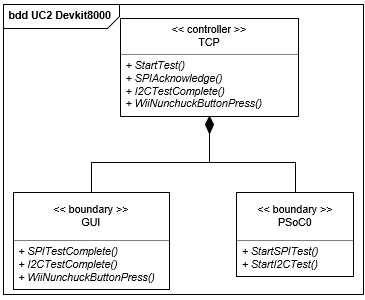
\includegraphics[] {Systemarkitektur/images/DevKit8000ClassDiagram}
	\caption{Klassediagram for Devkit 8000}
	\label{fig:klasseDevkit}
\end{figure}

% ---------------PSoC0 Applikationsmodel-----------------------------
\subsubsection{Applikationsmodel for Nunchuck Polling Software}

\begin{figure}[H]
	\centering
	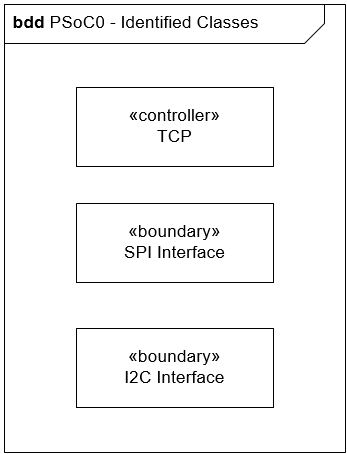
\includegraphics[scale=0.8]{Systemarkitektur/images/KlasseIdentifikationPSoC0.png}
	\caption{Klasseidentifikation for PSoC0}
	\label{fig:klasseidentifikationPSoC}
\end{figure}

På figur \ref{fig:klasseidentifikationPSoC} ses klasse identifikation for Nunchuck Polling Software. Der er til Nunchuck Polling Software for use case 2 identificeret tre klasser: \textit{Test Communication Protocol (TCP)}, \textit{SPI Interface}, og \textit{I2C Interface}.

\textit{TCP} er en controller. Denne klasse har til ansvar at eksekvere funktionalitet relevant til use case 2. \textit{SPI Interface} repræsenterer SPI grænsefladen til systemets SPI bus. \textit{I2C Interface} repræsenterer grænsefladen til systemets I2C bus.

På figur \ref{fig:sekvensPSoC0SPITest}, \ref{fig:sekvensPSoC0I2CTest} og \ref{fig:sekvensPSoC0NunchuckTest} ses sekvensdiagrammer for Nunchuck Polling Software. Sekvensdiagrammerne er blevet opdelt i de 3 tests der gennemføres i use casen; SPI, I2C og Nunchuck kommunikations tests.

\begin{figure}[H]
	\centering
	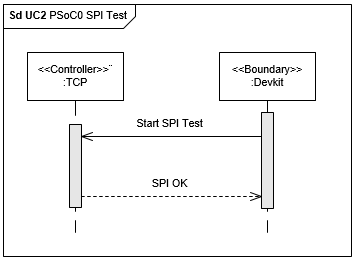
\includegraphics[width=.8\textwidth] {Systemarkitektur/images/SDPSoC0SPITest}
	\caption{Sekvensdiagram for PSoC0 SPI test}
	\label{fig:sekvensPSoC0SPITest}
\end{figure}

På figur \ref{fig:sekvensPSoC0SPITest} ses, at Devkittet sender en besked til kontrolklassen via \textit{SPI Interface} for at påbegynde SPI testen. Efter et bestemt timeout interval, læser Devkittet resultatet af SPI testen, igen via \textit{SPI Interface} grænsefladen.

\begin{figure}[H]
	\centering
	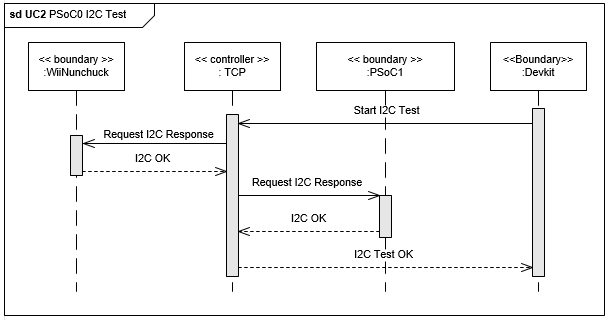
\includegraphics[width=\textwidth] {Systemarkitektur/images/SDPSoC0I2CTest}
	\caption{Sekvensdiagram for PSoC0 I2C test}
	\label{fig:sekvensPSoC0I2CTest}
\end{figure}

På figur \ref{fig:sekvensPSoC0I2CTest} ses, at Devkittet starter I2C testen, ved at sende en besked til \textit{TCP} klassen. \textit{TCP} klassen anmoder herefter om et acknowledge fra slaverne, via \textit{I2C Interface} grænsefladen, fra Nuchucken og PSoC1. Når disse enheder har svaret med et I2C OK er testen gennemført. Efter et bestemt timeout interval, læser Devkittet resultatet af I2C testen, via \textit{I2C Interface} grænsefladen.

\begin{figure}[H]
	\centering
	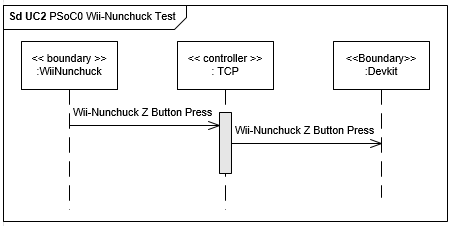
\includegraphics[width=\textwidth] {Systemarkitektur/images/SDPSoC0NunchuckTest}
	\caption{Sekvensdiagram for PSoC0 Nunchuck test}
	\label{fig:sekvensPSoC0NunchuckTest}
\end{figure}

På figur \ref{fig:sekvensPSoC0NunchuckTest} ses sekvensdiagrammet for Wii-Nunchuck testen. Devkittet sender en \textit{Start Nunchuck Test} besked til \textit{TCP} klassen, hvorefter testen startes. \textit{TCP} klassen anmoder om input data fra Nunchuck via \textit{I2C Interface} grænsefladen, hvorefter devkittet efter et bestemt timeout aflæser test resultatet.

\begin{figure}[H]
	\centering
	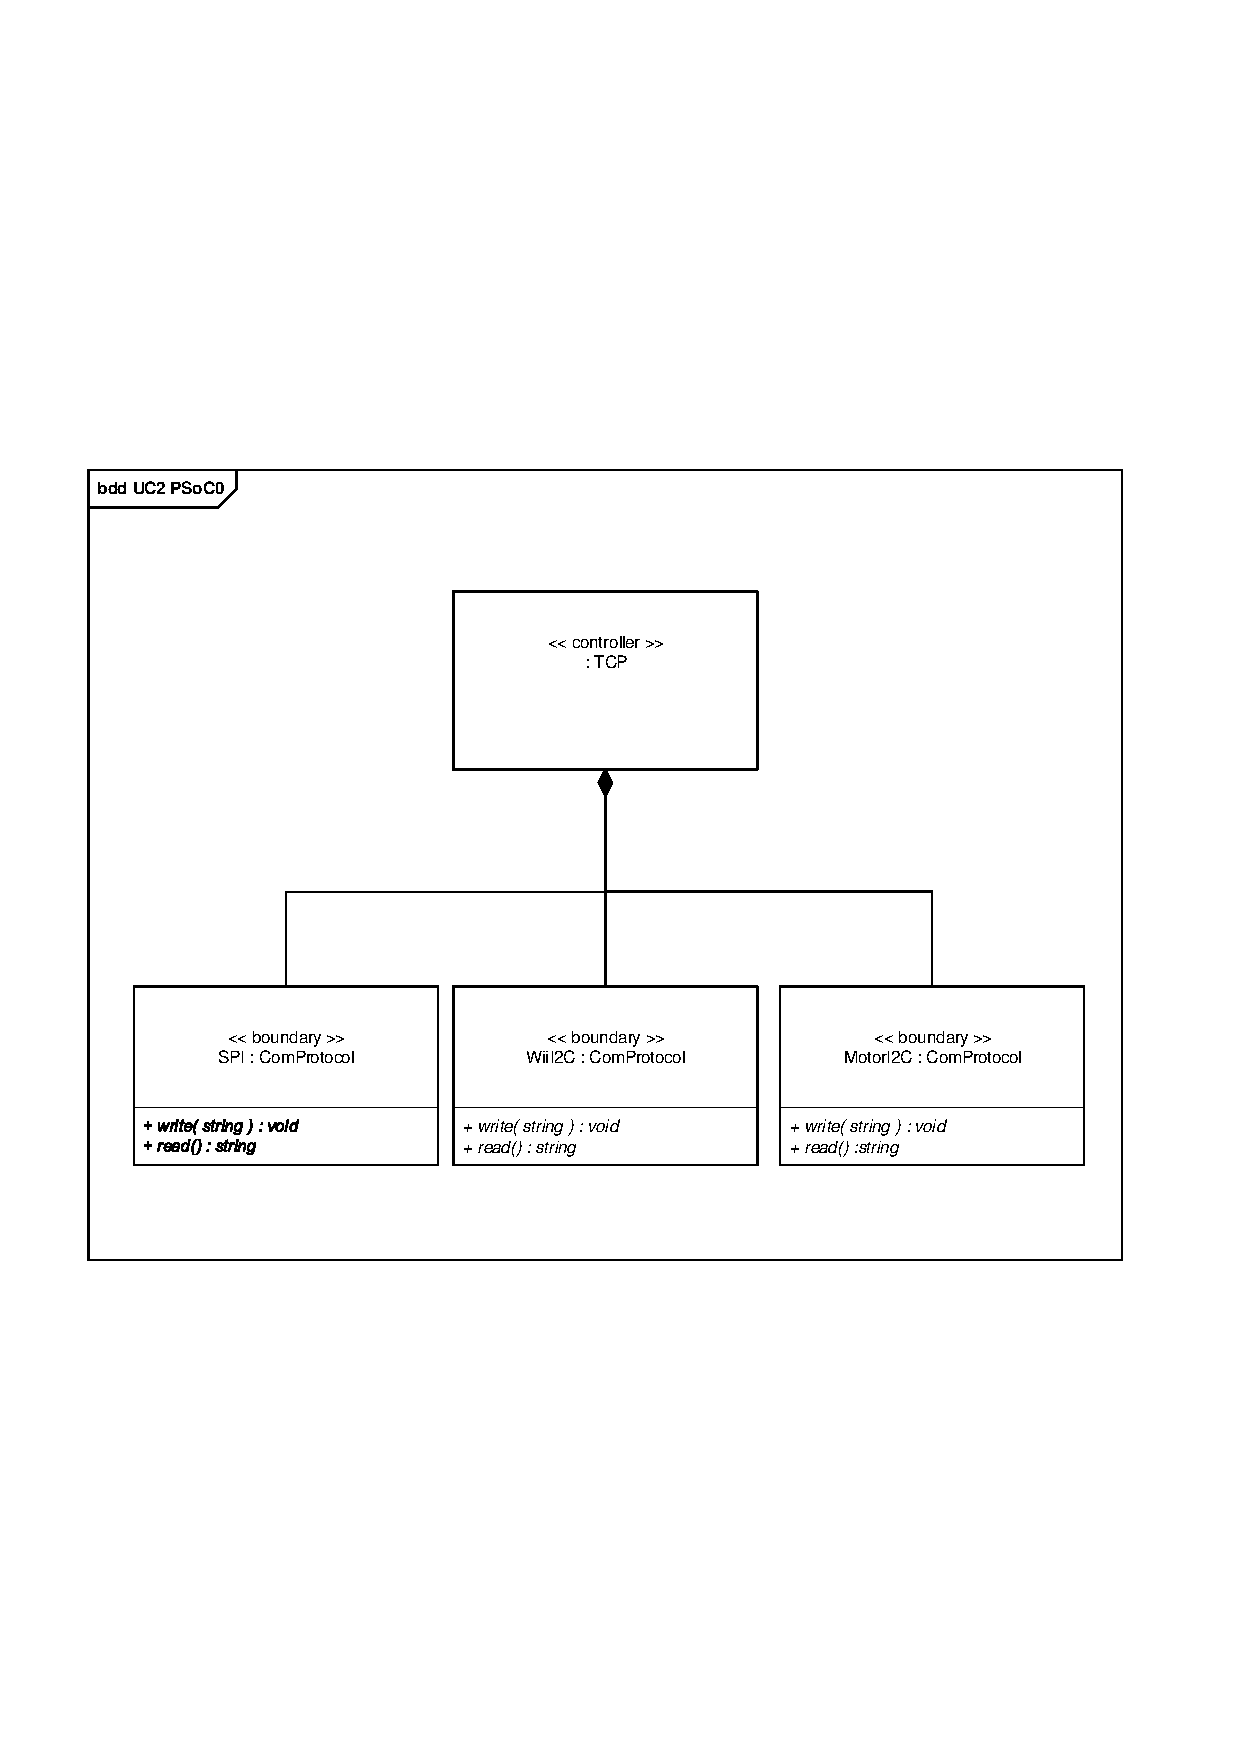
\includegraphics[width=\textwidth]{Systemarkitektur/images/klassediagramPSoC0}
	\caption{Klassediagram for PSoC0}
	\label{fig:klassePSoC0}
\end{figure}

På figur \ref{fig:klassePSoC0} ses det endelige klassediagram, hvor metoderne er udledt af sekvensdiagrammet, figur \ref{fig:sekvensPSoC0NunchuckTest}. Her kan det ses at \textit{TCP} klassen skal kunne bede om tilbagemelding for I2C bussens slaver via \textit{I2C Interface} grænsefladen. \textit{SPI Interface} grænsefladen skal kunne starte de relevante tests for use casen, samt aflæse resultaterne.

% ---------------PSoC1 Applikationsmodel-----------------------------
\subsubsection{Applikationsmodel for Motor Control Software}

\begin{figure}[H]
	\centering
	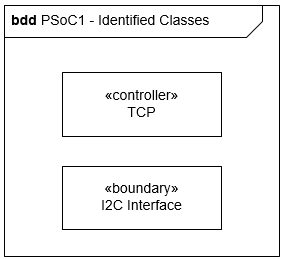
\includegraphics[scale=0.8]{Systemarkitektur/images/KlasseIdentifikationPSoC1.png}
	\caption{Klasseidentifikation for PSoC1}
	\label{fig:klasseidentifikationPSoC1}
\end{figure}

På figur \ref{fig:klasseidentifikationPSoC1} ses klasse identifikation for Motor control Software. Der er til Motor Control Software for use case 2 identificeret to klasser: 
\textit{Test Communication Protocol (TCP)} og \textit{I2C Interface}.

\textit{TCP} er en controller. Denne klasse har til ansvar at eksekvere funktionalitet relevant til use case 2. \textit{I2C Interface} repræsenterer grænsefladen til systemets I2C bus.

Sekvensdiagrammet for interaktion mellem de identificerede klasser ses på figur \ref{fig:sekvensPSoC1I2CTest}.

\begin{figure}[H]
	\centering
	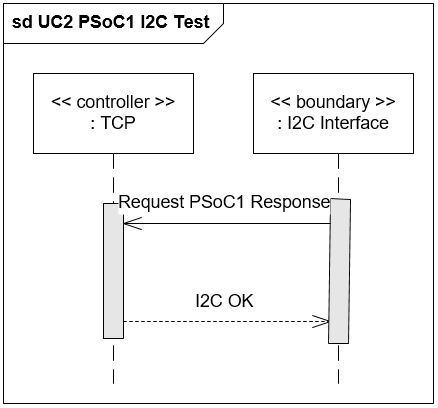
\includegraphics[width=.8\textwidth] {Systemarkitektur/images/SDPSoC1I2CTest}
	\caption{Sekvensdiagram for PSoC1}
	\label{fig:sekvensPSoC1I2CTest}
\end{figure}

På figur \ref{fig:sekvensPSoC1I2CTest} ses det at \textit{I2C Interface} grænsefladen anmoder om respons fra \textit{TCP} klassen for at bekræfte om I2C slaven kan kommunikeres med. Hvis dette er tilfældet sendes der I2C OK tilbage til boundaryklassen.  

\begin{figure}[H]
	\centering
	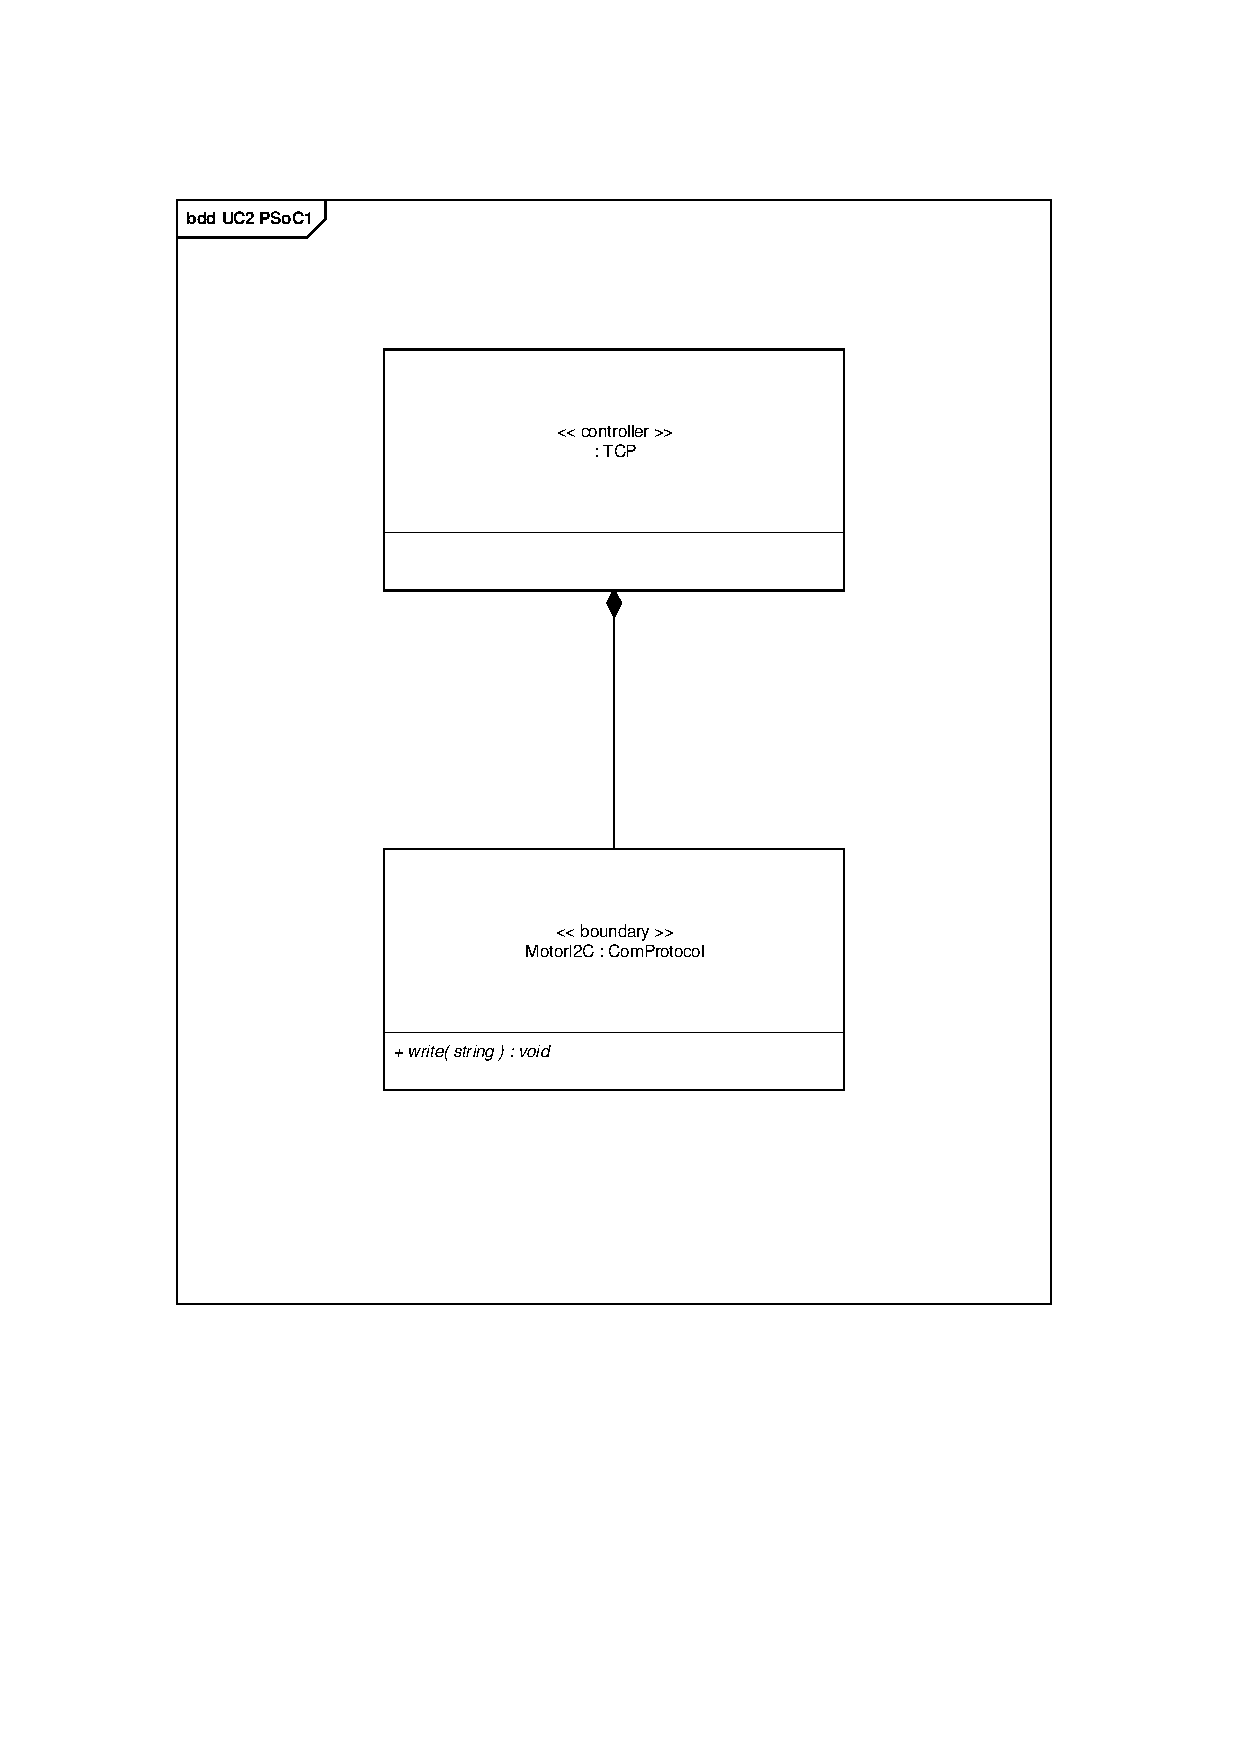
\includegraphics[width=.5\textwidth]{Systemarkitektur/images/klassediagramPSoC1}
	\caption{Klassediagram for PSoC1}
	\label{fig:klassePSoC1}
\end{figure}

Fra sekvensdiagrammet på figur \ref{fig:sekvensPSoC1I2CTest} udledes det endelige klassediagram som ses i figur \ref{fig:klassePSoC1}.

\section{Samlede Klassediagrammer}
Fra de detaljerede applikationsmodeller for use case 1- og 2, er der udledt samlede klassediagrammer for hver individuel CPU i systemet. Disse er med til at identificere konceptuelle klasser og funktionaliter der skal overvejes i implementation og design af systemet, og har altså fungeret som et udgangspunkt til resten af udviklingsprocessen.\newline\noindent
Figur \ref{fig:CompleteClassDiagramDevKit8000}, \ref{fig:CompleteClassDiagramPSoC0}, \ref{fig:CompleteClassDiagramPSoC1}, og \ref{fig:CompleteClassDiagramPSoC2} vises de samlede klassediagrammer for hver CPU.\newline\noindent
For disse klassediagrammer er der konceptuelle klasser som gentager sig selv. Alle klassediagrammer har én klasse af typen \textit{controller}. Disse klasse indeholder alt funktionalitet der er nødvændig for at kunne implementere systemets Use Cases. Yderligere bliver klasserne \textit{I2C Interface} samt \textit{SPI Interface} gentaget. Disse repræsenterer klasser for de tilsvarende bustyper, I2C og SPI, og bruges af softwaren til at sende og modtage data på disse busser.\newline\noindent
På figur \ref{fig:CompleteClassDiagramDevKit8000} ses det at DevKit8000 controlleren skal have funktionalitet til start af system test, i relation til Use Case 2. For at kunne udføre dette kommunikerer den med grænsefladen Graphical User Interface (\textit{GUI}), for at kunne vise resultater til brugeren. Desuden skal controlleren kommunikere med grænsefladen \textit{SPI Interface}, for at sende data ud til til resten af systemet via SPI bussen.

\begin{figure}[H]
	\centering
	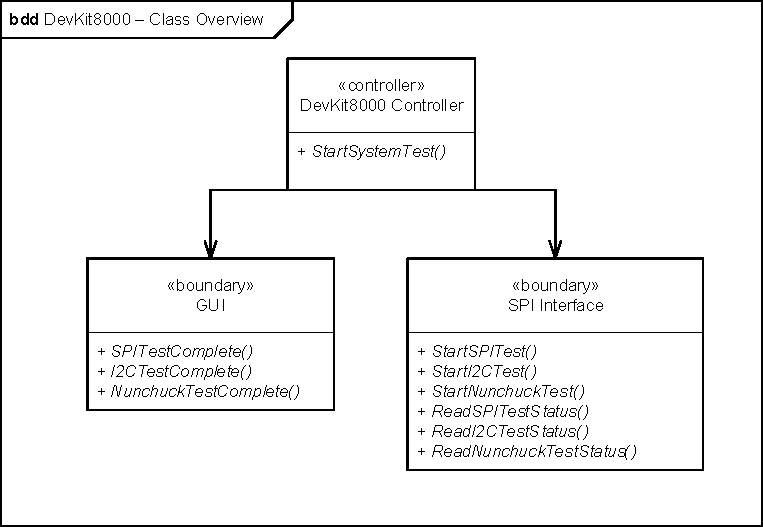
\includegraphics[width=\textwidth] {Systemarkitektur/images/CompleteClassDiagramDevKit8000}
	\caption{Samlet Klassediagram for DevKit8000}
	\label{fig:CompleteClassDiagramDevKit8000}
\end{figure}

På figur \ref{fig:CompleteClassDiagramPSoC0} ses det at PSoC0 controlleren skal have funktionalitet til at starte tests af systemets busser. Yderligere skal den også kunne dekode og kalibrere data der kommer fra Nunchuck. I relation til disse funktionaliteter skal den kunne modtage og sende data på systemets I2C og SPI busser.

\begin{figure}[H]
	\centering
	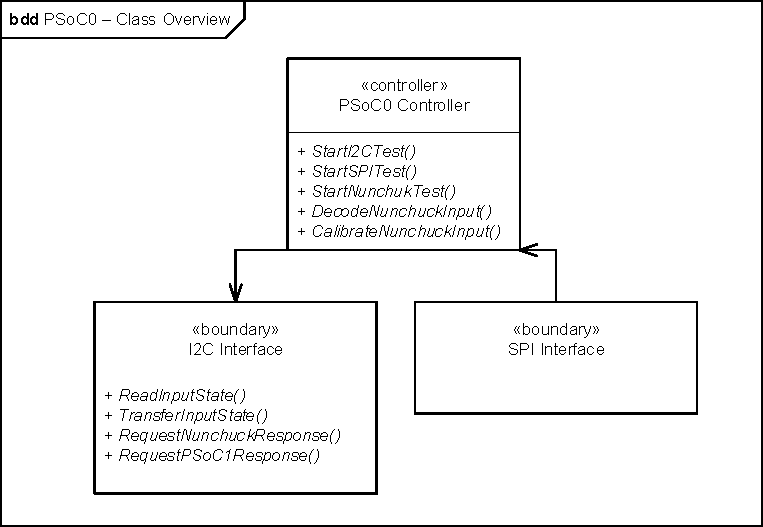
\includegraphics[width=\textwidth] {Systemarkitektur/images/CompleteClassDiagramPSoC0}
	\caption{Samlet Klassediagram for PSoC0}
	\label{fig:CompleteClassDiagramPSoC0}
\end{figure}

På figur \ref{fig:CompleteClassDiagramPSoC1} ses det at PSoC1 controlleren kommunikerer med grænsefladerne \textit{I2C Interface}, \textit{Motor Control} samt \textit{PSoC2}. Controlleren skal kunne regulere fart på systemets motorstyring, for at kunne styre kanonen. Desuden skal den kunne sende en affyringsbesked til \textit{PSoC2}. For at regulere fart og affyre kanonen, skal controlleren kunne aflæse Nunchucken's tilstand fra \textit{I2C Interface}.
\begin{figure}[H]
	\centering
	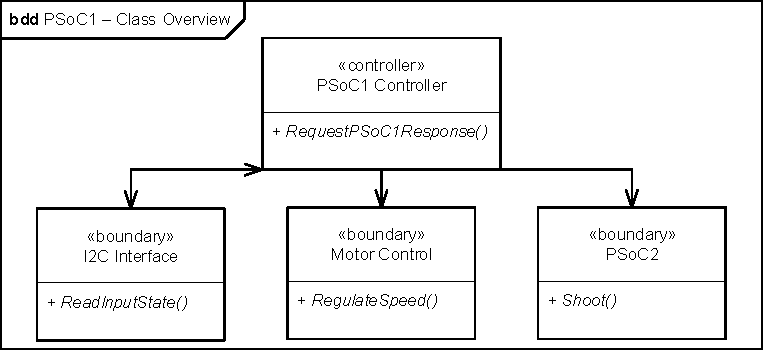
\includegraphics[width=\textwidth] {Systemarkitektur/images/CompleteClassDiagramPSoC1}
	\caption{Samlet Klassediagram for PSoC1}
	\label{fig:CompleteClassDiagramPSoC1}
\end{figure}

På figur \ref{fig:CompleteClassDiagramPSoC2} ses det at PSoC2 skal have funktionalitet til at aktivere afskydning, som gøres ved at kommunikere med grænsefladen \textit{Projectile Launcher}. Afskydningen aktiveres af grænsefladen \textit{PSoC1}.
\begin{figure}[H]
	\centering
	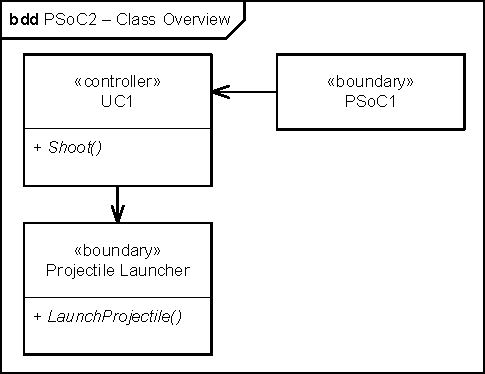
\includegraphics[width=\textwidth] {Systemarkitektur/images/CompleteClassDiagramPSoC2}
	\caption{Samlet Klassediagram for PSoC2}
	\label{fig:CompleteClassDiagramPSoC2}
\end{figure}

\section{Kommunikationsprotokoller}
\label{afsnit:kommunikationsprotokoller}
I dette afsnit beskrives de kommunikationsprotokoller der anvendes til at sende data mellem systemets komponenter på de anvendte bustyper - I2C og SPI. På figur \ref{fig:kommunikationsOverblik} ses hvilke bustyper der anvendes mellem systemets komponenter. 

\begin{figure}[H]
	\centering
	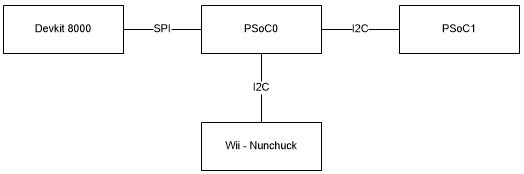
\includegraphics[width=\textwidth] {Systemarkitektur/images/anvendtebustyper}
	\caption{Forbindelser mellem systemets komponenter}
	\label{fig:kommunikationsOverblik}
\end{figure}

\subsection{SPI Protokol}
\label{afsnit:spiprotokol}
Til kommunikation mellem Devkittet og PSoC0 anvendes der \textit{Serial Parallel Interface (SPI)}. SPI-forbindelsen består af fire signaler. Et af signalerne er \textit{slave select} (SS). Det muliggør kommunikation med flere slaver. Selve dataen sendes via signalerne \textit{Master Out Slave In} (MOSI) og \textit{Master In Slave Out} (MISO). Det foregår ved \textit{Full Duplex}, hvor der altid sendes i begge retninger på én gang. Hvis der kun ønskes at sende i én retning, kan der sendes 0'er i den anden retning. Derudover er der en \textit{Clock} (SCLK), som sørger for at kommunikationen er synkron. I forhold til timing er det vigtigt, at både master og slave anvender samme \textit{Timing Mode}, som styres af to bit, \textit{SPI Clock Polarity Bit} (CPOL), som bestemmer om clock'en starter højt eller lavt, og \textit{SPI Clock Phase Bit} (CPHA), som afgør om data samples på clock'ens rising- eller falling edge. I dette projekt anvendes \textit{Timing Mode 3}, hvor clock'en starter høj og sampler på rising edge. \\
De kommandoer, der i projektet sendes via SPI, består af 8 bit. \\
På tabel \ref{tabel:spiKommandoType} ses SPI-protokollen. Til venstre på tabellen ses navnet på de kommandoer, der sendes. Alle kommandoer med "TEST" i navnet sendes fra Devkit8000 til PSoC0 via MOSI. De resterende kommandoer er svar på de forskellige tests, som sendes via MISO fra PSoC0 til Devkit8000. Det er værd at lægge mærke til, at det er bevidst, at der ikke er en kommando for SPI\_FAIL. Da SPI-forbindelsen ikke testes på PSoC0, men ved at PSoC0 sender \textit{SPI\_OK} tilbage til Devkit8000 via SPI-forbindelsen. Dermed kan det først afgøres om SPI-forbindelsen fungerer korrekt, når Devkit8000, modtager (eller ikke modtager) succes-beskeden fra PSoC0. \\


\begin{table}[H]
	\centering
	\resizebox{\textwidth}{!}{%
		\begin{tabular}{llll}
			\hline
			\multicolumn{1}{|l|}{Kommandotype}                                & \multicolumn{1}{l|}{Beskrivelse}                        & \multicolumn{1}{l|}{Binær Værdi} & \multicolumn{1}{l|}{Hex Værdi} \\ \hline
			\rowcolor[HTML]{CBCEFB} 
			{\color[HTML]{000000} START\_SPI\_TEST}                           & {\color[HTML]{000000} Sætter PSoC0 i 'SPI-TEST' mode}   & 1111 0001                        & 0xF1                           \\
			START\_I2C\_TEST                                                  & Sætter PSoC0 i 'I2C-TEST' mode                          & 1111 0010                        & 0xF2                           \\
			\rowcolor[HTML]{CBCEFB} 
			\begin{tabular}[c]{@{}l@{}}START\_NUN-\\ CHUCK\_TEST\end{tabular} & Sætter PSoC0 i 'NUNCHUCK-TEST' mode                     & 1111 0011                        & 0xF3                           \\
			SPI\_OK                                                           & Signalerer at SPI-testen blev gennemført uden fejl      & 1101 0001                        & 0xD1                           \\
			\rowcolor[HTML]{CBCEFB} 
			I2C\_OK                                                           & Signalerer at I2C-testen blev gennemført uden fejl      & 1101 0010                        & 0xD2                           \\
			I2C\_FAIL                                                         & Signalerer at der skete fejl under I2C-testen           & 1100 0010                        & 0xC2                           \\
			\rowcolor[HTML]{CBCEFB} 
			NUNCHUCK\_OK                                                      & Signalerer at NUNCHUCK-testen blev gennemført uden fejl & 1101 0011                        & 0xD3                           \\
			NUNCHUCK\_FAIL                                                    & Signalerer at der skete fejl under NUNCHUCK-testen      & 1100 0011                        & 0xC3                          
		\end{tabular}
	}
	\caption{Kommandotyper der anvendes ved SPI kommunikation}
	\label{tabel:spiKommandoType}
\end{table}

For at aflæse en besked fra SPI-slaven, skal slaven først klargøre dens SPI-transfer buffer. Dette gøres ved, at SPI-masteren sender en commandotype til slaven, som derefter tolker kommandotypen, og eksekverer kommandoen, hvor SPI-transfer bufferen bliver sat. Imens dette sker, venter SPI-masteren i et bestemt stykke tid, for at sikre at transfer-bufferen når at blive sat. På figur \ref{figure:SDSpiReadSlave} ses et sekvensdiagram der illustrerer dette. 

\begin{figure}[H]
	\centering
	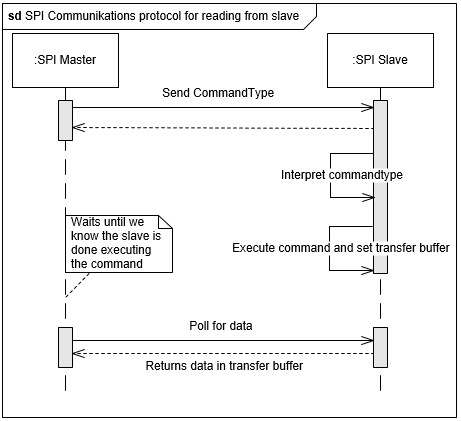
\includegraphics[]{SystemArkitektur/images/SDSpiSlaveRead}
	\caption{Sekvensdiagram for at læse fra SPI-slaven}
	\label{figure:SDSpiReadSlave}
\end{figure}


\subsection{I2C Protokol}
\label{afsnit:I2CProtokol}

I2C\cite{I2C} er en bus bestående af to ledninger. Den ene ledning bruges som databus og navngives \textit{Serial Data Line} (SDA). Den anden ledning bruges til clock signalet, der synkroniserer kommunikationen, og navngives \textit{Serial Clock Line} (SCL). Enheder på I2C bussen gør brug af et master-slave forhold til at sende og læse data. En fordel ved I2C bussen er at netværket kan bestå af multiple masters og slaver, hvilket udnyttes i dette system da tre I2C komponenter skal sende data mellem hinanden.

I2C gør brug af en integreret protokol der anvender adressering af hardware-enheder for at identificere hvilken enhed der kommunikeres med. På tabel \ref{table:I2CAddress} ses addresserne tildelt systemets PSoCs.

\begin{table}[H]
	\centering
	\begin{tabular}{lllllllll}
		\hline
		\multicolumn{1}{|l|}{I2C Adresse bits} & 7                        & 6                        & 5                        & 4 & 3 & 2 & \multicolumn{1}{l|}{1} & \multicolumn{1}{l|}{0 (R/W)} \\ \hline
		\rowcolor[HTML]{CBCEFB} 
		{\color[HTML]{000000} PSoC0}           & {\color[HTML]{000000} 0} & {\color[HTML]{000000} 0} & {\color[HTML]{000000} 0} & 1 & 0 & 0 & 0                      & 0/1                          \\
		PSoC1                                  & 0                        & 0                        & 0                        & 1 & 0 & 0 & 1                      & 0/1                         
	\end{tabular}
	\caption{Adresser der anvendes på I2C bussen}
	\label{table:I2CAddress}
\end{table}

Den integrerede I2C protokol sender data serielt i pakker af 8-bit (1 byte). På figur \ref{fig:I2CTimingDiagram} ses et timing diagram for aflæsning af 1 byte. Figuren er et udsnit fra databladet for en LM75, der anvender fire faste addressebits, tre vilkårlige bit og en read/write bit. Her ses at transmissionen af data begynder med en addresse-byte til slaven efterfulgt en acknowledge til masteren og herefter sendes en data-byte. 

\begin{figure}[H]
	\centering
	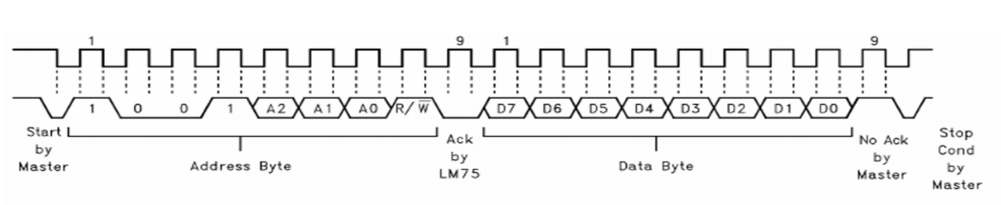
\includegraphics[width=\textwidth] {Systemarkitektur/images/I2CTimingDiagram}
	\caption{Timing Diagram af 1-byte I2C aflæsning}
	\label{fig:I2CTimingDiagram}
\end{figure}

Goofy candygun gør brug af I2C protokollen via PSoC's I2C \textit{Application Programming Interface} (API). Ved brug af denne API er der blevet udviklet en kommunikationsprotokol mellem systemets PSoCs, som gør det muligt at sende kommandoer og data.

Da I2C dataudveksling sker bytevist, er kommunikations protokollen opbygget ved, at kommandoens type indikeres af den første modtagne byte. Herefter følger \textit{N}-antal bytes som er kommandoens tilhørende data. \textit{N} er et vilkårligt heltal og bruges i dette afsnit når der refereres til en mængde data-bytes der sendes med en kommandotype.

Kommandoens type definerer antallet af databytes modtageren skal forvente og hvordan disse skal fortolkes. På figur \ref{fig:I2CProtokolEksempel} ses et sekvensdiagram der, med pseudo-kommandoer, demonstrerer forløbet mellem en I2C afsender og modtager ved brug af kommunikations protokollen.

\begin{figure}[H]
	\centering
	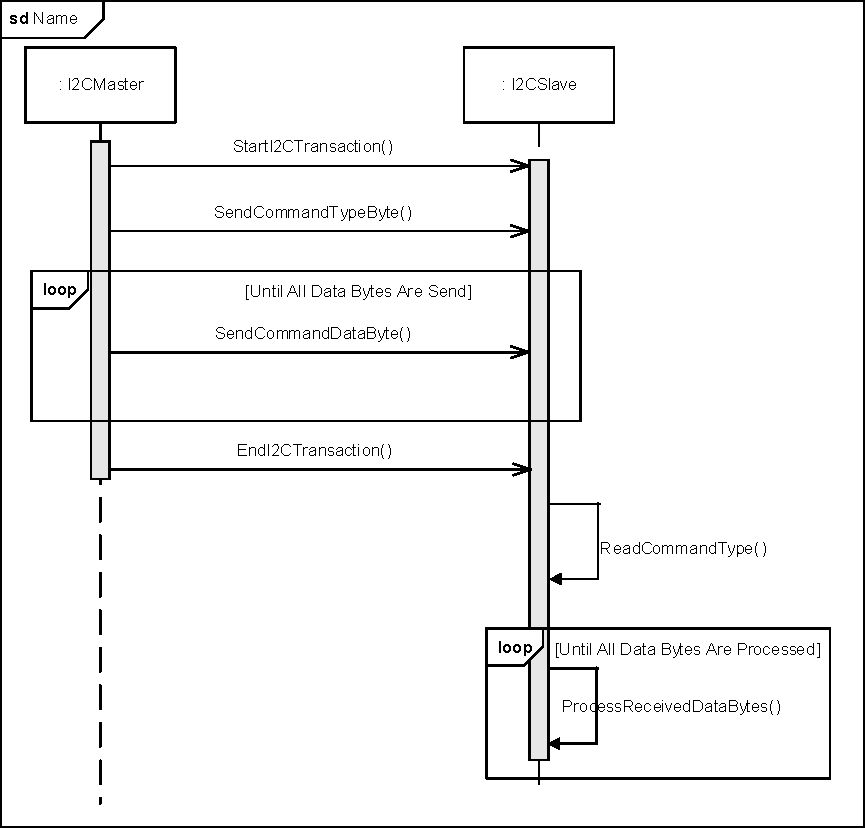
\includegraphics[width=\textwidth] {Systemarkitektur/images/I2CProtocol}
	\caption{Eksempel af I2C Protokol Forløb}
	\label{fig:I2CProtokolEksempel}
\end{figure}

På figur \ref{fig:I2CProtokolEksempel} ses at afsenderen først starter en I2C transaktion, hvorefter typen af kommando sendes som den første byte. Efterfølgende sendes \textit{N} antal bytes, afhængig af hvor meget data den givne kommandotype har brug for at sende. Efter afsluttet I2C transaktion læser I2C modtageren typen af kommando, hvor den herefter kan fortolke \textit{N} antal modtagne bytes afhængig af den modtagne kommandotype.

På tabel \ref{table:I2CKommandoer} ses de definerede kommandotyper og det tilsvarende antal af bytes der sendes ved dataveksling.

\begin{table}[H]
	\centering
	\resizebox{\textwidth}{!}{
		\begin{tabular}{lllll}
			\hline
			\multicolumn{1}{|l|}{Kommandotype}    & \multicolumn{1}{l|}{Beskrivelse}                                            & \multicolumn{1}{l|}{Binær Værdi} & \multicolumn{1}{l|}{Hex Værdi} & \multicolumn{1}{l|}{Data Bytes}                                                                                         \\ \hline
			\rowcolor[HTML]{CBCEFB} 
			{\color[HTML]{000000} NunchchuckData} & {\color[HTML]{000000} Indeholder aflæst data fra Wii Nunchuck controlleren} & 0010 1010                        & 0xA2                           & \begin{tabular}[c]{@{}l@{}}Byte \#1 Analog X-værdi\\ Byte \#2 Analog Y-værdi\\ Byte \#3 Analog Buttonstate\end{tabular} \\
			I2CTestRequest                        & Anmoder PSoC0 om at starte I2C-kommunikations test                          & 0010 1001                        & 0x29                           & Ingen databyte                                                                                                          \\
			\rowcolor[HTML]{CBCEFB} 
			I2CTestAck                            & Anmodning om at få en I2C OK besked fra I2C enhed                           & 0010 1000                        & 0x28                           & Ingen databyte                                                                                                         
		\end{tabular}
	}
	\caption{Kommandotyper der anvendes ved I2C kommunikation}
	\label{table:I2CKommandoer}
\end{table}

Kolonnerne "Binær Værdi" og "Hex Værdi" i tabel \ref{table:I2CKommandoer} viser kommandotypens unikke tal-ID i både binær- og hexadecimalform. Denne værdi sendes som den første byte, for at identificere kommandotypen. 

\section{Brugergrænseflade}


Ved hjælp af en brugergrænseflade, kan systemtesten styres fra DevKit8000.
Brugergrænsefladen er opbygget ud fra sekvensdiagrammet figur \ref{fig:SystemTestOverviewSequenceDiagram},
ud fra dette kunne brugergrænsefladen skitseres som figur \ref{fig:GUISkitse}.
Grænsefladen mellem DevKit8000 og PSoC0 er en SPI-bus som ses på figur \ref{fig:IBD}, og brugergrænsefladen er koblet til DevKit8000 ved hjælp af en interfacedriver.
Brugergrænsefladen skal sende startsekvensen til interfacedriveren, hvorefter dette sendes til PSoC0 og videre ud i systemet.
Brugergrænsefladen skal aflæse svaret fra systemtesten og printe dette ud i en konsol.

\begin{figure}[H]
	\centering
	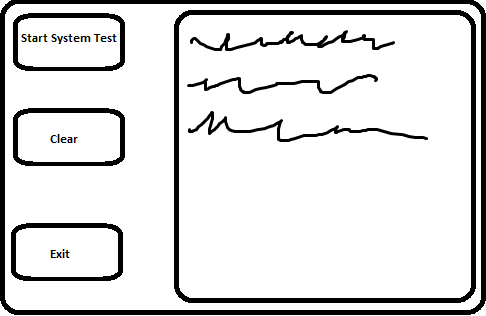
\includegraphics[width=\textwidth] {Systemarkitektur/images/GUISkitse}
	\caption{Skitse af brugergrænseflade}
	\label{fig:GUISkitse}
\end{figure}


Brugergrænsefladen er designet ud fra den sekventielle struktur i usecase 2, se afsnit \ref{afsnit:FUC2}. Dette er løst ved hjælp af Event-Driven Programming.
Denne model drives ved hjælp af events, som i dette tilfælde aktiveres af brugeren ved knaptryk. Knapperne vil blive tildelt forskellige funktionaliteter, der faciliterer systemtesten.

Et alternativ kunne være trådbaseret design. Interfacedriveren kunne oprettes som en seperat tråd fra GUI'en, der ville køre den samme funktionalitet. Dette ville være unødvendigt i forhold til den sekvetielle struktur i systemet. Kompleksiteten i dette design ville være overvældende i forhold til den ønskede funktionalitet og blev derfor fravalgt.

